\documentclass[12pt, a4paper]{article}
\pagestyle{plain}
\renewcommand{\baselinestretch}{1.27} 
\linespread{1}
\usepackage[margin=1in]{geometry}
\usepackage{cite}
\usepackage{float}
\usepackage{graphicx}
\usepackage[%  
    colorlinks=true,
    pdfborder={0 0 0},
    linkcolor=red
]{hyperref}
\usepackage{caption}
\captionsetup{font=footnotesize}
\usepackage{amsmath}
\usepackage{tablefootnote}
\usepackage{subcaption}
\usepackage{natbib}
\usepackage{filecontents}
\usepackage{setspace}
\doublespacing
\usepackage{indentfirst}
\usepackage{amsmath}
\usepackage{float}
\usepackage{tabularx}
\usepackage{xcolor}
\usepackage{booktabs}
\usepackage{array}
\usepackage{geometry}
\usepackage{pdflscape}
\usepackage{amsfonts}
\usepackage{breqn}
\newcolumntype{C}[1]{>{\centering}p{#1}}
\usepackage{pdfpages,verbatim }
\usepackage{enumitem}
\usepackage{blindtext}
\usepackage{hyperref}
\hypersetup{colorlinks,linkcolor={blue},citecolor={blue},urlcolor={red}}  
\usepackage[english]{isodate}
\usepackage{amssymb}
\newcommand\blfootnote[1]{%
\begingroup
\renewcommand\thefootnote{}\footnote{#1}%
\addtocounter{footnote}{-1}%
\endgroup
}

\title{Central Bank Digital Currency and Cryptocurrency in Emerging Markets }
\date{}
\begin{document}

\maketitle
\begin{abstract}

\noindent Blockchain technology has opened up the possibility of digital currency, smart contracts and much more applications including the launch of central bank digital currencies (CBDC). However, literature about the effect of CBDC with the presence of cryptocurrency in an emerging market economy seems to be left behind. In this paper, we introduce a New Keynesian - Dynamic Stochastic General Equilibrium (NK-DSGE) model to examine the implications of CBDC and cryptocurrency in an open economy for emerging markets. In our model, cryptocurrency is implemented as a form of deposit in banks where bankers can also receive deposits from abroad. Lastly, CBDC is introduced as payment and saving instrument. We find that cryptocurrency has a crucial role in banking sectors and a significant effect on the dynamic of foreign debt which is deeply important for emerging markets. We also conduct optimal monetary policy under different scenarios. Hence, we uncover that a flexible rate in CBDC can affect the responses of the monetary rate and can reinforce the conventional monetary policy to achieve the central bank's targets.
   
   


\noindent\textbf{Keywords:} Central bank digital currency, Cryptocurrency, Open-economy,\\ Financial frictions, Optimal monetary policy
\vspace{0in}\\
\noindent\textbf{JEL Codes:} E50, F30, F31, G15, G18, G23\\

\bigskip
\end{abstract}

\setcounter{page}{0}
\thispagestyle{empty}
\clearpage
\section{Introduction}

In the last 10 years, we have observed a significant development of digital currencies backed by blockchain technology. Blockchain technology opens up the possibility of decentralized digital currencies, commonly called cryptocurrency or digital money. Currently, the size of the cryptocurrency market reaches more than 1000 billion USD and continues to grow. However, there are several issues with using cryptocurrencies such as Bitcoin and others from the macroeconomic and financial stability perspective. The main concerns include the high volatility in price, liquidity and credibility of issuers. Holders of cryptocurrencies also wobble the value of their savings following the cryptocurrency volatility in price, which will then lead to fluctuations in consumption, investment and hours worked and cause macroeconomic fluctuation and financial instability. Therefore, the regulation of crypto is highly recommended by the IMF to many countries (\cite{imffintech}, \cite{imf2020digital}).

Central banks, within their mandate, have a responsibility to control price stability as well as ensure financial stability, and they can only do this through their fiat currency or financial regulations on fiat currency-related instruments. However, cryptocurrencies or crypto assets, due to their nature of decentralization, are not controlled by central banks or central institutions. A potential solution for this matter is the introduction of central bank digital currencies (CBDC). In nutshell, CBDC are digital tokens and have no difference compared to cryptocurrencies except for being controlled by central banks. If stablecoin is regulated, the differences between CBDC and stablecoin are negligible. As a result, central banks in both developed and emerging market economies are studying the optimal adoption of CBDC intensively. According to \cite{auer2021cbdcs}, more than 86\% of central banks are doing research on the advantages and disadvantages of issuing CBDC. Among many central banks who are actively conducting research on this matter, some remarkable examples include China’s Digital Currency Electronic Payment from The People's Bank of China (PBOC) and the Digital Euro from The European Central Bank (ECB) as well as the Digital Dollar—or Fedcoin from The Federal Reserve (FED). Having said that, looking at Figure \ref{cbdcmap}, we can see that most of the countries are working intensively on their CBDC. Until now, only the Bahamas and Nigeria have already issued their own CBDC. Nevertheless, the optimal design for CBDC and its effects on the economy are still being studied intensively.

\begin{figure}[H]
  \hspace{-0.7cm}
  \caption{Global status of CBDC development}
	\centering
	\centerline{\includegraphics[scale=0.3 ]{cbdc.jpg}}
	\subcaption*{Source: CBDC Tracker (cbdctracker.org)}
	\label{cbdcmap}
\end{figure}

Among many theoretical models about digital currency (both cryptocurrency and CBDC) , some of them includes \cite{auer2020technology}, \cite{auer2021cbdcs}, \cite{auer2021central}, \cite{agur2022designing}, \cite{schilling2019currency}, \cite{benigno2019monetary}, \cite{brunnermeier2019equivalence}, \cite{ikeda2020digital}, \cite{kumhof2021central}, \cite{minesso2022central}, \cite{kumhof2018central}, \cite{kumhof2021central}, \cite{engert2017central}, \cite{fernandez2021central}. The main focuses of these papers are the macroeconomic effect of CBDC and optimal designs for banking. However, most papers concentrate on the view of large economies such as the U.S. and EU but leave a gap in the literature for the implication for the small emerging economy as well as developing countries. According to \cite{chen2022cbdcs}, central banks in developing countries also join the race of issuing their own CBDC following the FED or ECB. However, as pointed out by \cite{imf2020toward}, emerging markets and developing economies need some distinguished features in dealing with policy challenges which are called Integrated Policy Framework by the IMF. Thus, studying the implications of CBDC in emerging markets also requires modifications in the model structures modelling. Hence, this paper is aimed to fill the gap in the literature on CBDC as well as cryptocurrencies for emerging markets.

In this paper, we assess the implications of CBDC in an emerging market economy with financial sectors and the presence of a cryptocurrency. Thus, the paper contributes to the fast-growing literature on CBDC as well as cryptocurrencies. I conduct the study by building up the small open economy model of \cite{aoki2016monetary}. However, this model differs in some aspects. First, I include the presence of cryptocurrencies similar to \cite{sockin2018model} and \cite{asimakopoulos2019new}. However, I allow the banking sector to take cryptocurrencies as a deposit following \cite{murakami2021cryptocurrencies}. This extension aims to reflect the fact that the banking sector started incorporating cryptocurrencies into its balance sheet. Moreover, due to strict capital control policies in many emerging markets, I assume that the trade in foreign currency-denominated assets (i.e deposits or bonds) can only be conducted through the banking system but not the households. Second, I introduce CBDC as a digital instrument inside a menu of the monetary assets following \cite{agur2022designing} and \cite{minesso2022central}. Besides the concerns on decentralization, CBDC differs from cryptocurrencies in the sense that cryptocurrencies are mainly considered financial assets for investment purposes rather than payment instruments for daily activities. The digital aspect of CBDC brings up two main advantages: it has no storage cost compared to cash and can be mounted up easily. Also, due to the nature of CBDC, we can consider it as a mixture of a payment instrument and a financial asset. First, CBDC can be liquid anytime similar to cash. Second, it also has features such as bonds and deposits as it can be a saving asset with an interest rate. Third, it is perfectly safe in the sense that it is backed by central banks. Therefore, it is not subject to a decentralized risk such as the issuer of digital assets can control the supply for their benefit. Lastly, CBDC is also not subject to partial financial risks such as bank deposits. As pointed out by \cite{keister2020discussion}, CBDC might be helpful for the bank run scenario by central bank credibility. Hence, the CBDC is particularly useful during financial distress with liquidity problems.

%In this model, the central bank issues cash and CBDC, which can be used for payment and distributed synchronously. Moreover, our model tries to include as many technical features in CBDC design as possible especially the hybrid feature of using for payment and saving. However, I leave the possibility for households to hold foreign CBDC out of the model.  We calibrate our model using the parameter assumptions of \cite{aoki2016monetary} and \cite{minesso2022central}. In general, with this model, I try to address the following questions.

%1) How does the CBDC affect macroeconomic dynamics? 

%2) Are the designs of CBDC matter for the economy? 

%3) What is the effect of CBDC on the banking sector with foreign debt?

%4) What are the effect of CBDC and cryptocurrency in emerging markets?

The results of this paper shed some light on a growing body of literature on digital assets, CBDC. Some of these results are in line with the existing literature. In particular, I also find that the introduction of CBDC does not affect the domestic macroeconomic variables significantly when we fix the return on CBDC as 1. With the fixed return of CBDC as 1, we assume that CBDC is only used for payment but not for saving. However, different from the results of \cite{murakami2021cryptocurrencies}, I find that allowing bankers to hold cryptocurrencies can mitigate the negative effect of some shocks because the return of cryptocurrency is partly shielded from changes in the policy rate. This allows the banking sector to have more alternatives for funding sources. The main reason for our contrast can be traced back to the fact that I implement a different form of the utility function and assume the household can hold cash, CBDC and cryptocurrency at the same time compared to two types of households in  \cite{murakami2021cryptocurrencies}. This gives rise to a substitution effect for households in responding to shocks. Surprisingly, with CBDC and cryptocurrencies, we observe significant changes in the dynamic of foreign debt. Cryptocurrency and CBDC seem to help reduce the dependence on foreign debt which is important for an emerging market economy. However, the model is not able to depict the high volatility of cryptocurrency. Thus, our cryptocurrency should be referred to as a stablecoin and our results should be considered with caution. Moving forward, alternative designs of CBDC reveal many more interesting observations. Using optimal welfare monetary policy analysis, I find that CBDC can provide an additional tool for central banks and sustain the movement of the nominal rate in achieving the central bank's targets. Last but not least, a flexible rate in CBDC return can also affect the responses in the banking sector. Finally, this paper also contributes to the literature on structured models in CBDC and cryptocurrency. To the best of my knowledge, there is yet a model to include CBDC and cryptocurrency for an emerging market model with financial frictions.

\textbf{Related literature:}Various studies have studied the implications of cryptocurrencies and CBDC. Because the body of literature is too vast to enumerate, I can only provide a partial list.

In cryptocurrency, most of the theoretical models are the partial equilibrium and asset-pricing models. \cite{bohme2015bitcoin} presents a non-technical paper to sum up cryptocurrency's principles and properties. They also discuss the potential risks and issues of cryptocurrency. \cite{fernandez2019can} study the competition among privately-issued currencies.\cite{athey2016bitcoin} and \cite{garratt2018bitcoin} study the behaviour and mechanism of Bitcoin-to-Dollar exchange rate. \cite{schilling2019currency} present the model with Bitcoin and the U.S. Dollar which allow both currencies to be used for transactions. \cite{sockin2018model} build the model with cryptocurrency producers for clearing conditions and allow cryptocurrency to fulfil transactions for goods. \cite{benigno2019monetary} assume that cryptocurrency can be a global currency. They use a two-country model with a global stablecoin that can be traded freely. The results suggest that the unified interest rate makes the global cryptocurrency and the domestic currency to be indifferent. \cite{baughman2022global} study the welfare effects of global stablecoins which correlate with sovereign currencies. Their results suggest the demand for global stable coins is low which is contradict the findings of \cite{benigno2019monetary}.

In CBDC, the literature has been growing swiftly last 5 years. \cite{boar2021ready} provide a survey of CBDC adoption around the world. In the study on CBDC, the first strand is about the effect of CBDC on commercial banks as well as its financial inclusion. Theoretically, CBDC is a hybrid instrument and can serve as an interest-bearing substitute for commercial bank deposits. \cite{foster2021digital} and \cite{andolfatto2021assessing} suggest that the idea of accessing fintech for everyone with CBDC can accelerate financial inclusion and enlarge the digital economy. \cite{andolfatto2021assessing}  also argue that the benefit of CBDC may outweigh the competitive pressure for commercial banks and the situation may end up with an expansion in deposits. \cite{chiu2019bank} extend the study of \cite{andolfatto2021assessing} by allowing commercial banks to hold CBDC to meet their reserve requirements. They find that the return on CBDC has a significant effect on commercial banks' activities. \cite{fernandez2021central} study the bank run scenario with CBDC.

The second strand is about the function of central banks with CBDC on monetary policy and financial stability. \cite{barrdear2016macroeconomics} build an NK-DSGE where newly issued CBDC can be exchanged one-for-one with government debt. They find that CBDC can have a positive effect on GDP growth and mimic the drop in GDP for a liquidity demand shock because it fulfils the need for a flight to safety for households. \cite{cukierman2019welfare} argue that central banks need CBDC to preserve the effectiveness of monetary policy with the presence of cryptocurrencies. Moreover, it also has a welfare effect on central banks. Nevertheless, \cite{cukierman2019welfare} does not provide a theoretical model to rationalize arguments. \cite{schilling2020central} claim that issuing CBDC cause an impossible trilemma for central banks on efficiency, financial stability and price stability. The paper concludes that only two targets can be achieved at once. \cite{keister2020discussion} also conduct an intensive study about CBDC effects on government policy in periods of financial distress. They claim that CBDC provides an alternative means of payment to bank deposits but is not subject to the risk of bank runs because CBDC is backed by the central bank. This reduces the severity of the bank run. By appropriately choosing the interest rate on CBDC to make it more attractive in times of stress, the central bank can stabilise the financial system better and respond more effectively. 

The remainder of the paper is organized as follows. Section 2 characterizes a model for an open economy with CBDC, cryptocurrency,  financial frictions, nominal rigidities, and foreign debt in banking sectors. Section 3 analyzes the simulation results. Section 4 concludes.

\section{Model}
Below I introduce the baseline model for the paper. In general, the main framework is a NK-DSGE model with financial frictions under the style of \cite{gertler2010financial} and \cite{gertler2011model} (henceforth GK). I extend the banking sector following \cite{aoki2016monetary} (henceforth ABK) in which we allow the possibility of funding from foreigners in the financial sector. Moreover, we allow bankers to hold cryptocurrencies on their balance sheets. The model focuses on modelling financial intermediaries in which bankers face endogenously determining balance sheet constraints. Compared to the GK model, our model does not have capital utilization, quantitative easing rule or price indexation. 

On the household side, different from \cite{murakami2021cryptocurrencies}, we assume there is only one type of representative household that has physical cash, cryptocurrencies, and CBDC in their utility function. The representative household consists of a continuum of households of measure unity following DSGE literature. In each period, we assume the portion $(1-f)$ of the population are workers, and the other portion $f$ are bankers. Each banker remains their work in the banking sector with probability $\chi$ in the following period. Therefore, in every period,  ($1-\chi )f$ bankers become workers. This is important to prevent banks from accumulating an infinite amount of net worth, making financial frictions irrelevant. Because we also assume a fraction of ($1-\chi )f$ workers choose to be bankers every period,  the proportion of bankers in the population remains unchanged. In the banking sector, each of them runs a bank and their profits go to the households. Deposits from the households are assumed to go to banks that the households do not own. Lastly, we assume that each household shares the idiosyncratic risk. The creation of cryptocurrency is modelled following \cite{sockin2018model} and \cite{asimakopoulos2019new}. Each period corresponds to a quarter. In a nutshell, the model includes six types of agents: households, banking sectors, intermediate goods producers,  retailers, capital producers, cryptocurrency producers, and a government that conducts monetary policy following a standard Taylor rule and has CBDC and cash as her liability. As the paper relies heavily on the structure of ABK, we use the same notations as ABK when it is convenient.

\subsection{Households}
First, different from the GK model, households can also directly invest in firms' equity with an extra cost $\chi^h(K^h_t,K_t)$. This cost can be interpreted as management cost for their investment. At the same time, bankers can also hold equity. For simplicity, we assume the function form of the cost as, $\chi^h(K^h_t,K_t) = \frac{\varkappa^h}{2}\left(\frac{K^h_t}{K_t}\right)$. Because we assume that bankers are more productive in conducting investments, a positive parameter $\varkappa^h$ governs the disadvantage of households relative to professional bankers in financing firms.

Households can hold deposits into banking sectors, $D_t$, cryptocurrency, $Cryp_{t}$, and CBDC, $DC_{t}$. Following \cite{asimakopoulos2019new}, \cite{murakami2021cryptocurrencies} and \cite{minesso2022central}, I include all three instruments inside the utility function. As mentioned by \cite{woodford2003interest}, households can derive utility from liquidity service because they need liquid instruments for payment. Hence, utility parameters follow their liquidity level. 


\begin{align}
   U_t=  E_t \sum_{t=0}^{\infty} \beta^t\left[ ln\left(C_t-\zeta_{0}\frac{H_t^{1+\zeta}}{1+\zeta}\right) -\chi_{DC}\varrho\left(\frac{M_t}{M_t+DC_t},\Gamma\right) +\mu^C\left(\frac{Cryp_t^{1-\sigma^c}}{1-\sigma^c}\right)\right] 
\end{align}
\begin{align*}
&\text{s.t.}  \nonumber\\
  & C_t + D_{t} + B_t + Q_t K^h_t  + M_t + DC_t + Cryp_t +\chi^h(K^h_t,K_t) \\   
 & = w_t H_t + \frac{R_{t-1}}{\pi_t} B_{t-1}+ \frac{R^D_{t-1}}{\pi_t} D_{t-1} + (Z_t+ \lambda Q_t) K^h_{t-1} + \epsilon^m M_{t-1} + \frac{R^{DC}_{t-1}}{\pi_t} DC_{t-1} +\frac{R^{C}_{t-1}}{\pi_t} Cryp_{t-1}  +\Pi_t 
\end{align*}
where $C_t$ denotes total consumption, $w_t$ denotes the real hourly wage and $H_t$ is total labour, $K^h_{t-1}$ stands for the physical capital at time t, $R^D_{t-1}$ is the risk-free nominal interest rate for deposits calculated using available information at time t, and $\Pi_t$ is total  transfers from either the government or firms (profit). $R^{DC}_{t-1}$ is the CBDC nominal interest rate and $R^C_{t-1}$ is the return on cryptocurrency. $\epsilon^m$ is the storage cost for holding cash. $Z_t$ and $Q_t$ denotes productivity and price of household capital respectively.

Stem from \cite{agur2022designing} and \cite{minesso2022central}, we assume that only cash and CBDC are used for paying for consumption goods. Hence, households encounter a Hotelling linear city where they minimize the spread between the available forms of liquid tools for payment and their preferences. In our model, we assume the representative agent as the household\footnote{Allowing for heterogenous agents in the sense of preference is another approach to model the heterogeneity in preference of payment instruments}. However, the representative household is a unit continuum of atomistic households with heterogeneous preferences on payment instruments which are uniformly distributed. Intuitively, a part of the population prefers cash relative to CBDC and the other part prefers CBDC relative to cash. For example, young people might like CBDC more as it can be used for many digital services while old and middle age people might like using cash because of its anonymity. For getting those features into our model, we implement a utility loss function where the function depends on the share of instruments households like the least. For example, if a person dislikes using cash but moves to use cash as the return on CBDC decreases, they face a utility loss for rebalancing their payment method.

Similar to \cite{minesso2022central}, I introduce the re-balancing payment utility loss function, $\varrho\left(\frac{M_t}{M_t+DC_t},\Gamma\right)$, and  $\varrho(0)=0$,  $\varrho(.)' > 0$,  $\varrho(.)'' > 0$. $\Gamma$ is the function's global minimum and the household’s preferred mix of payment instruments. Because we set a global minimum of function as $\left(\frac{M_t}{M_t+DC_t}\right) = \Gamma$, $\Gamma$ can also interpreted as the fraction of household members in steady state who prefer cash over CBDC. If the global minimum is achieved, there is no utility loss from using that mix. However, depending on many other factors, a household's optimal decisions might be different from $ \Gamma$ in responding to shocks.
\subsection{Production Sectors}
\begin{align}
    Y_{t}(i)=\Gamma_t(i),
\end{align}
where $Y_{t}(i)$ is the combination of an intermediate input using differentiated intermediate goods. The CES aggregator of all retail products and a demand function of the representative final-good firm for the generic input i is the following:

\begin{align}
   Y_{t}=\left[\int_0^1 Y_{t}(i)^{\frac{\epsilon-1}{\epsilon}}di\right]^{\frac{\epsilon}{\epsilon-1}}
\end{align}

\begin{align}
  Y_{t}(i)= \left(\frac{P_{t}(i)}{P_{t}}\right)^{-\epsilon} Y_{t}
\end{align}

Because the profits for final-good producers are zero in equilibrium, it implies the relationship between the price level and retail prices as:
\begin{align}
    P_{t}=\left[\int_0^1P_{t}(i)^{1-\epsilon}di\right]^{\frac{1}{1-\epsilon}}
\end{align}

Retailer (i) chooses $ P_{t}(i)$, expressed in terms of the domestic CPI, to maximize her future discounted profit.

\begin{align}
   E_t{\sum_{t=0}^\infty\beta^t\frac{\lambda_{t}}{\lambda_0}\left[\frac{ P_{t}(i)-MC_{t}}{P_t}Y_{t}(i)-\frac{AC_t(i)}{P_t}\right]}
\end{align}
with $MC_{t}$ is the marginal costs of the retail sector and adjustment costs for setting prices, $AC_t(i)$, are defined as:
\begin{align}
    AC_t(i)=\frac{\Omega_P}{2}\left(\frac{P_{t}(i)}{P_{t-1}(i)} -\bar{\pi}\right)^2 P_{t} Y_{t}
\end{align}

A change in retail prices requires quadratic adjustment costs $AC_t(i)$ in nominal term à la \cite{rotemberg1982sticky} where they change prices with respect to  $\bar{\pi}$. The NK Philips curve is expressed as\footnote{Small letter refers to relative to price level}:
\begin{align} 
 mc_{t} =p_{t}(\frac{\epsilon-1}{\epsilon})+   \frac{\Omega_P}{\epsilon}(\pi_{t}-\bar\pi)\pi_{t}-\beta\left(\frac{\lambda_{t+1}}{\lambda_t}\pi_{t+1}(\pi_{t+1}-\bar\pi)\frac{p_{t+1}Y_{t+1}}{p_{t}Y_{t} }\right) 
\end{align}

Given the symmetric assumption, the aggregate output, $Y_t$ can be written in the following form:
\begin{align}
    Y_t= A_t \left(\frac{K_{t-1}}{\alpha_K}\right)^{\alpha_K} \left(\frac{X_{t}}{\alpha_X}\right)^{\alpha_X}
    \left(\frac{H_{t}}{1-\alpha_K-\alpha_M}\right)^{1-\alpha_K-\alpha_X}
\end{align}
where $K_{t-1}$, $X_t$ and $H_t$ are aggregate capital stock, imported materials and labour from households. To ensure the model solution, we consider $K_{t-1}$ as cumulative capital predetermined by the end of the $t-1$ and is used for production at time t.

Instead of allowing households to produce capital, in line with GK and ABK, capital producers purchase the final goods and non-depreciated capital to produce capital goods which are bought later by intermediate firms. However, she is subject to an investment adjustment cost.

\begin{align}
\max E_t \sum_{t=0}^\infty\beta^t\frac{\lambda_{t}}{\lambda_0}[q_t K_t-(1-\delta)q_t K_{t-1}-I_t]
\end{align}s.t
\begin{align}
K_t = (1-\delta) K_{t-1} +\left[1-\frac{\kappa_I}{2}\left(\frac{I_t}{I_{t-1}}-1\right)^2\right]I_t
\end{align}

On the foreign demand, we assume exogenous foreign demand and characterize it as a function of the relative price of the export and foreign income. Intuitively, the foreign demand increases with their purchasing power by either a drop in the cost of the export or an increase in income.

\begin{align}
    EX_t=\left(\frac{P_t}{s_tP^*_t}\right)^{\varphi} Y^*_t
\end{align}
with $s_t$ as the real exchange rate and $Y^*_t$ is exogenous foreign demand  from the perspective of the small open economy.

\subsection{Financial Intermediates}
In this part, we quickly present the banking sector (bankers). Bankers have three sources of funding to make their capital investment to producers. There are domestic deposits, $D_t$, foreigner deposits, $D^*_t$, and cryptocurrencies, $Crypt_t$. The foreign deposits are converted into domestic currency with an exchange rate of $s_t$. However, we assume that borrowing from foreigners is costly in terms of resources to take into risk premium on emerging markets' foreign debt accumulation, $\left(1+\frac{\varkappa_{b}}{2}\right)^2$. Hence, the flow of funds constraints for a representative bank are given as follows:
\begin{align}
   \left(1+\frac{\varkappa_{b}}{2} x^2_t\right)^2 Q_t K^b_t = N_t+ D_{t} +s_t D^*_t+ Cryp_t ,
\end{align}

As mentioned briefly above, businesses may receive two sources of capital. The first is from the household directly. The second is from the financial sector, $K^b_t$. Then the net worth is as follows:
\begin{align}
 {N}_{t}= \left({Z}_{t}+{Q}_{t}\, {\lambda}\right)\, {K}^{b}_{t-1}-\frac{ {D}_{t-1}\, {R}_{t-1}}{{\pi}_{t}}-\frac{s_t D^{*}_{t-1}{R^{*}}_{t-1}}{\pi^*_t} -\frac{ {Cryp}_{t-1}\, {R}^c_{t-1}}{{\pi}_{t}}
\end{align}
\subsection{Bankers Optimization}
At the begging of period t, bankers raise funds and purchase assets from the businesses. During this period, the banker decides whether to keep working as a banker (operating honestly) or divert assets. Deciding to keep being a banker means holding capital until the payoffs are realized and the banker fulfils the obligations to creditors. To divert means to secretly divert funds as much as a fraction $\theta$ of total assets away from investment in order to consume personally. 

We define $V_t$ as the bank's value function, which can be considered as the "market value" of bankers. $\theta$ is the fraction of diverted assets. Hence, the incentive constraint is as followed:
\begin{align}
    V_t(N_t)\geq \theta Q_t K^b_t
\end{align}
For convenience, the leverage ratio and Tobin's Q ratio are defined respectively.
\begin{align}
    \psi_t = \frac{V_t}{N_t}
\end{align}
 \begin{align}
 lev_t=\frac{Q_t K^b_t}{N_t}    
 \end{align}
     
 Under a perfect financial market, the incentive constraint always holds with equality to prevent an indefinitely asset expansion. However, in our model, banks are also subject to a terminal wealth maximization problem. Banks maximize the expected terminal wealth which is written in the recursive formulation.

\begin{align}
   V_t(N_t)= \max E_{t}\Lambda_{t;t+1}[ (1-\sigma)N_{t+1}+\sigma V_{t+1}(N_{t+1})]
\end{align}
We rewrite the problem in terms of Tobin's Q maximization\footnote{A detailed derivation of banks problem can be found in the appendix}.
\begin{align}
    & \psi_t = \max_{lev_t, x_t}\left(\mu_t lev_t  +\left(1+\frac{\varkappa_{b}}{2}lev_t^2 x_t \right)v_t +\mu_t lev_t x_t + \mu^c_t lev_t x^c_t \right)\\
    &\text{s.t.} \quad \nonumber \\
    &\psi_t  \geq \Theta(x_t, x^c_t)lev_t,
\end{align}
We define that  $\Omega_{t;t+1}$ is the stochastic discount factor of the banker. $\mu_t$  is the excess return
on capital over home deposits. $\mu^c_t$ is the cost advantage of cryptocurrency holdings over home deposits. $\mu^*_t$ is the cost advantage of foreign currency debt over home deposits or the deviation from real uncovered interest parity (UIP). $v_t$ is the marginal cost of deposits. All of the above terms are defined as follows.
\begin{align}
\mu_t=E_t\left[\Lambda_{t;t+1}\left(\frac{Z_{t+1}+\lambda Q_{t+1}}{Q_t} -R_{t,t+1} \right)\right] \\
\mu^*_t=E_t\left[\Lambda_{t;t+1}\left(R_{t+1} - \frac{s_{t+1}}{s_t}R^*_{t,t+1} \right)\right] \\
\mu^c_t=E_t\left[\Lambda_{t;t+1}\left(R_{t+1} - R^c_{t,t+1} \right)\right] \\
v_t=E_t\left[\Lambda_{t;t+1} R_{t+1}\right] \\
\Omega_{t+1} = \Lambda_{t;t+1}(1-\sigma + \sigma \psi_{t+1}) 
\end{align}



\subsection{Government and Central Bank}
The central bank determines the nominal interest rate with a Taylor rule, targeting CPI inflation and exchange rate stabilisation. Lastly, government expenditure is financed by lump-sum tax from households.
\begin{align}
    \left(\frac{{{R}_{t}}}{{\bar R}}\right)=  \left(\frac{{{R}_{t-1}}}{{\bar R}}\right)^{\rho_r} \left(\left(\frac{\pi_t}{\bar \pi}\right)^{\phi^\pi} \left(\frac{\Delta e_t}{\Delta e}\right)^{\phi^e}\right)^{1-\rho_r} exp(\epsilon^m_{t})
\end{align}
where $\Delta e_t = \frac{s_t\pi_t}{s_{t-1}\pi_t^*}$
\subsection{Parameterisation}
As mentioned above, parameter values are taken from \cite{aoki2016monetary}, \cite{minesso2022central}, \cite{asimakopoulos2019new}, and \cite{murakami2021cryptocurrencies}. Most of the important values are reported in Table \ref{calib}. Also, most parameters of the production and household sectors are relatively standard
in macroeconomic models. As we have no evidence of the elasticity of leverage on cryptocurrency, we set it equal to the elasticity of foreign borrowing. For banking sectors, we set ex-ante the steady-state leverage ratio to 4 and spread to 2\% annually. This results in a proportional transfer to the new bankers being 0.002 and the fraction of foreign borrowing accounts for 25\% of bank assets. In addition, the survival rate of the bankers is set as 0.972.

Notably, we assume the household prefer liquidity asset. We set the cryptocurrency sub-utility parameter to 0.0025. Moreover, as CBDC is assumed to be more efficient, we set $\mu^{DC}= \mu*1.1$ which means that it is 10\% more efficient than cash. The elasticity of substitution will follow the efficiency governing parameters as $\sigma^c= \sigma^m +(1-\Xi)\sigma^m$ and $\sigma^{DC}= \sigma^m $. $\Xi$ governs the liquidity level of the instrument. As cryptocurrency has a low liquidity level, we set it to 0.25 compared to a benchmark of 1 for cash.



\begin{table}[H]
\caption {\label{calib} Calibrated Parameter Values} 
%\begin{ruledtabular}
\begin{tabular}{lll}
 \hline
 \textbf{Parameter} & \textbf{Value}  &  \textbf{Description}  \\ 
 \hline
$\theta$ 	 & 	 0.401 	 & 	 elasticity of leverage wrt foreign borrowing\\
$\theta^c$ 	 & 	 0.401 	 & 	 elasticity of leverage wrt cryptocurrency\\
%$\theta_{0}$ 	 & 	 0.399 	 & 	 home bias in funding\\
$\sigma$ 	 & 	 0.94 	 & 	 survival probability\\
$\xi$ 	 & 	 0.0045 	 & 	 fraction of total assets brought by new banks\\
$\varkappa^{b}$ 	 & 	 0.0197 	 & 	 management cost for foreign borrowing\\
$\beta$ 	 & 	 0.985 	 & 	 discount rate\\
$\zeta$ 	 & 	 0.333 	 & 	 inverse of Frisch elasticity of labour supply\\
$\zeta_{0}$ 	 & 	 7.883 	 & 	 inverse of labour supply capacity\\
$\varkappa_{h}$ 	 & 	 0.0197 	 & 	 cost parameter of direct finance\\
$\alpha_{K}$ 	 & 	 0.30 	 & 	 cost share of capital\\
$\alpha_{M}$ 	 & 	 0.18 	 & 	 cost share of imported intermediate goods\\
$\lambda$ 	 & 	 0.98 	 & 	 one minus the depreciation rate\\
$\eta$ 	 & 	 9	 & 	 elasticity of demand\\
$\omega$ 	 & 	 0.667 	 & 	 Calvo parameter of price stickiness\\
$\kappa_{I}$ 	 & 	 0.667 	 & 	 cost of adjusting investment goods production\\
$\varphi$ 	 & 	 1.000 	 & 	 price elasticity of export demand\\
$\omega_P$ 	 & 	 52.450 	 & 	 slope of NKPC\\
$\chi_{DC}$ 	& 	 0.5	 & 	 Loading of payment instrument preferences in the utility function\\
$\rho_{DC}$ 	 & 	 0.01	 & 	 Substitution between payment instruments\\
$\epsilon^m$ 	 & 	 1 & 	storage cost\\
$\mu$ 	 & 	 0.5 & 	Cash efficiency\\
$\mu^{DC}$ 	 & 	 $\mu*1.1$ & 	CBDC efficiency\\
$\mu^{C}$ 	 & 	 0.0025 & 	Crypto efficiency\\
$\bar{A}$ 	 & 	 1.000 	 & 	 steady state productivity\\
$\rho_{i}$ 	 & 	 0.800 	 & 	 Taylor rule persistence\\
$\phi_{\pi}$ 	 & 	 1.500 	 & 	 Taylor rule response to inflation\\
$\phi_{\delta e}$ 	 & 	 0.3 	 & 	 Taylor rule response to depreciation rate\\
$\rho_{A}$ 	 & 	 0.900 	 & 	 TFP persistence\\
$\rho_{R*}$ 	 & 	 0.900 	 & 	 foreign interest rate persistence\\
$\rho_{Y*}$ 	 & 	 0.900 	 & 	 foreign income persistence\\
$\sigma_{i}$ 	 & 	 0.0025 	 & 	 standard deviation of interest rate shock\\
$\sigma_{i*}$ 	 & 	 0.0025 	 & 	 standard deviation of foreign interest rate shock\\
$\sigma_{A}$ 	 & 	 0.01 	 & 	 standard deviation of TFP shock\\

 \hline
\end{tabular}
%\end{ruledtabular}
\end{table}
\section{Numerical Simulations}
This section is aimed to illustrate the quantitative results of the paper. I mainly focus on the dynamic responses to these shocks: productivity shock (TFP), monetary policy shock, and foreign rate shock. I conduct analysis through the impulse response function step by step. First, I focus on the model's dynamics with and without the presence of cryptocurrency and CBDC. Second, I focus on the effect of alternative CBDC designs on the economy. Third, I conduct the optimal policy analysis for different versions of our model. Lastly, I also provide other results from the model in the Appendix.
\subsection{Baseline Results}

First, we consider the effect of a 1\% expansionary shock on total productivity in the domestic economy. A positive TFP shock creates an expansion of output on impact. Then, we investigate the effects of the introduction of CBDC and the presence of cryptocurrency in the banking sector. For doing that, I compare results from models in which we have different combinations of available assets in household hands. The Base model is our model with crypto, cash and CBDC. Lastly, the return on CBDC for the Base model will be fixed. Thus, CBDC is purely a payment instrument under the Base model. 

The reaction of variables to the positive TFP shock is relatively standard following other NK-DSGE models. Similar to output responses, investment and consumption increase following the TFP shock. Besides, working labour decreases following a positive productivity shock. To unload extra production as the production is more efficient, prices of goods decline which pushes inflation down. The central bank reacts to deflationary pressures by adapting the nominal interest rate downwards. Hence, the economy goes through a deterioration of its inflation rate. However, through UIP, the exchange rate is depreciating which makes imported goods more expensive relative to domestic goods. Therefore, as can be seen from an increase in the trade balance, exports are growing much faster than imports. This diminishes the effect of increasing imported prices (via exchange rate depreciation) on the composition of CPI prices.  The investment and consumption increase persistently after the shock but the trade balance only increases temporary and dissipates gradually over time. For the banking sector, the net worth of banks increases on impact. An increase in total productivity level improves intermediary balance sheets, which helps to reduce the spread even further. This results in a lower credit spread rate in the market due to a lower profit pressure for banks and high economic activity.



\begin{figure}[H]
    \hspace{-0.7cm}
	\centering
	\centerline{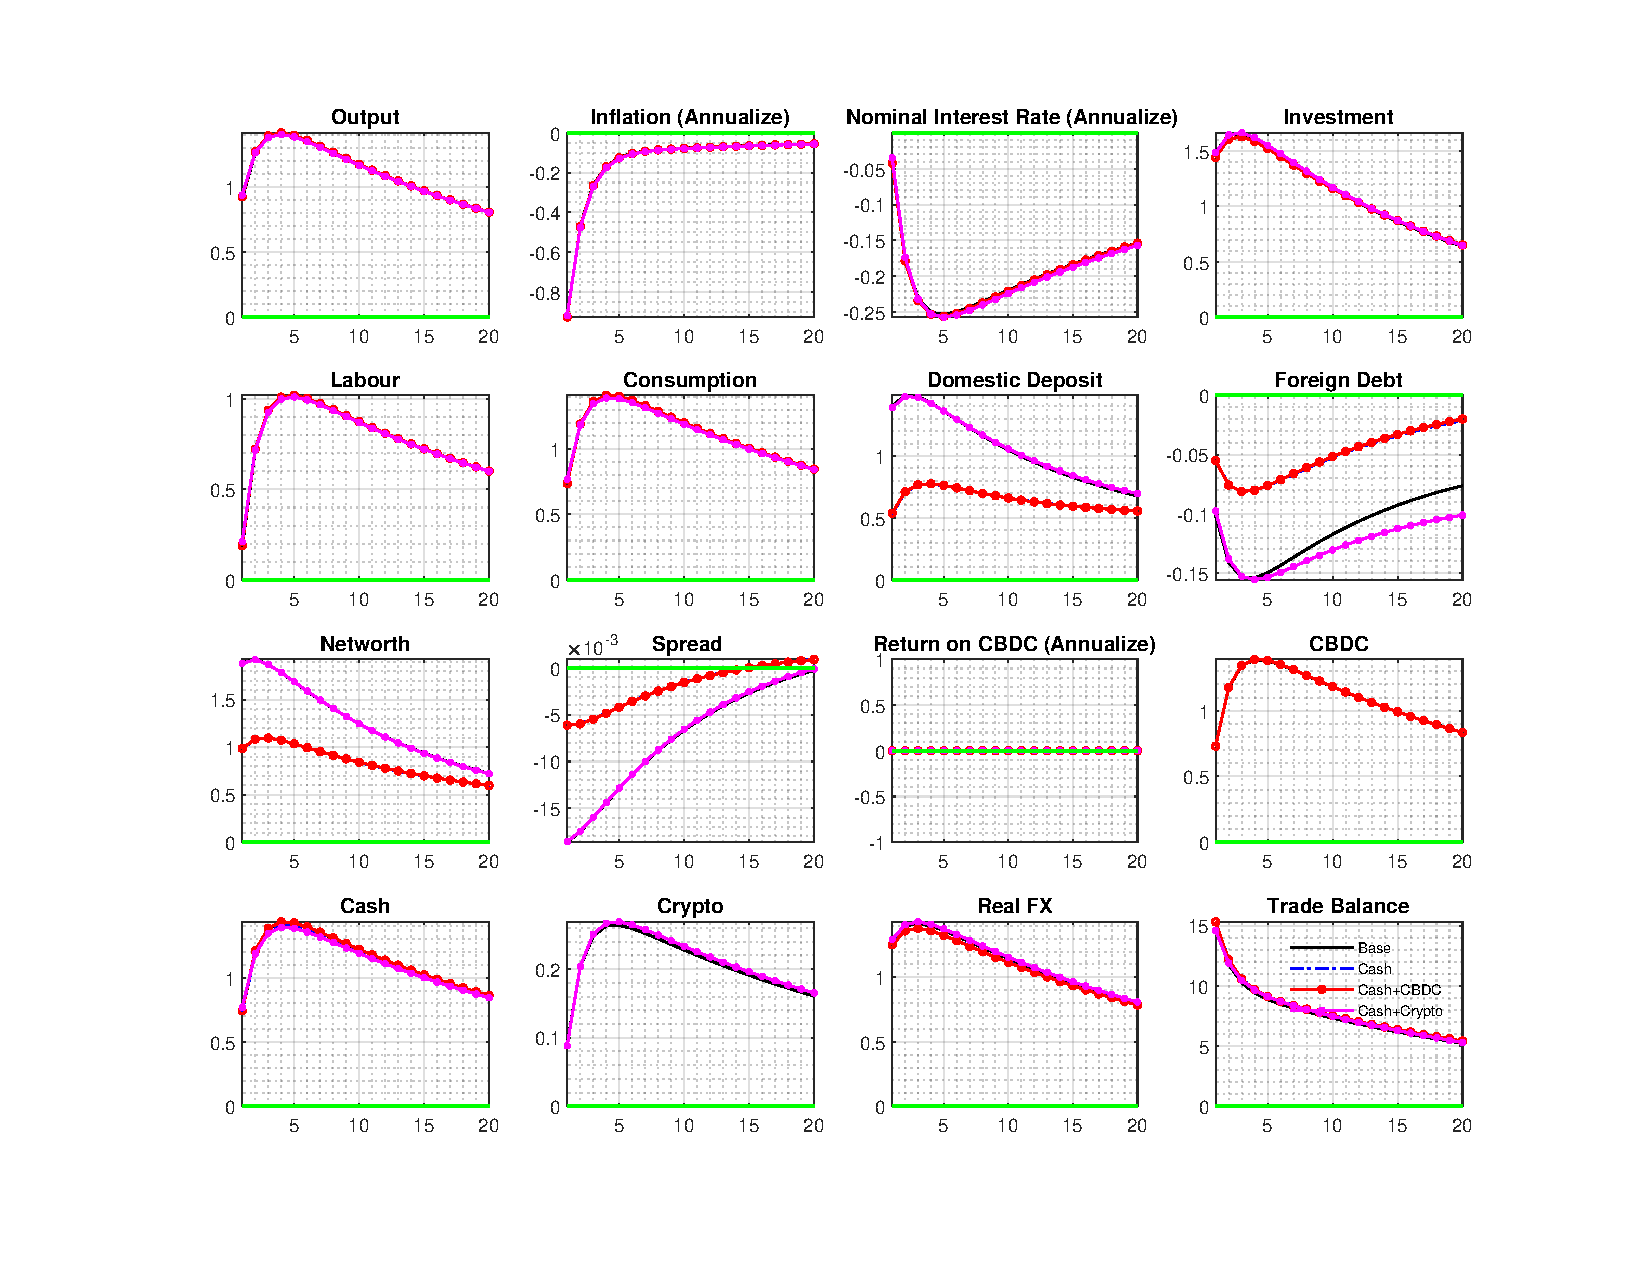
\includegraphics[trim = 0mm 23mm 0mm 18mm, clip, scale=0.97]{TFP_cashvs.pdf}}
	\caption{Response of selected variables to a 1\% expansionary total factor productivity shock in the domestic economy. All variables are expressed in percentage deviation from steady state.}
	\label{TFP}
\end{figure}



As can be seen from Figure \ref{TFP}, the introduction of CBDC seems to not generate huge differences compared to the model with only cash which is similar to the finding of \cite{minesso2022central}. As we impose CBDC and cash as payment instruments, this should not cause much difference in responses to shocks in other sectors. However, we find that the introduction of cryptocurrency can bring a significant effect on the banking sector. Both the net worth and spread react mostly double compared to the model without cryptocurrency. Moreover, foreign debt in the banking sector also reacts much more stronger compared to the model with only cash and CBDC. This may raise the concern of higher volatility in financial sectors for adapting cryptocurrency as an official financial instrument. This fact was not observed in \cite{murakami2021cryptocurrencies} which also implements cryptocurrency in the ABK model. This paper differs from \cite{murakami2021cryptocurrencies} by allowing only one kind of household that can optimally decide between cash, CBDC and cryptocurrency. Also, we implement a different setup of cryptocurrency inside the utility function. Hence, this might gives rise to the responses of the financial sector.

Now,  we consider the effect of 25 basic points contractionary shock of domestic monetary rate in Figure \ref{money}. Again, similar to TFP shock, the responses are also in line with other models. The shock leads to a contraction in output on impact. Contraction of output shows the standard recession effect by decreasing both investment and consumption and pushing down the inflation rate. This shock decreases consumption as it affects transmit through wealth effects as well as inter-temporal effects. As the real interest rate also increases, it reduces investment. The asset price, Tobin's q, drops significantly. The friction is between depositors (foreign and domestic) and bankers. First, banks receive deposits from households. Combined with their current net worth, they make a profit by lending this to intermediate firms. With an increase in monetary rate, both capital good value and investment surge because a higher nominal means that the rental income of capital is discounted heavily. However, banks have to suffer from the fluctuation in the asset price themselves. Hence, this causes an on-impact decrease in bank net worth.  Compensating for the risk of increasing leverage, banks need to increase profit by raising the lending rate to intermediate firms which increases the spread. However, due to a decreasing path of banks' leverage, the spread rises on impact and decreases over time. Therefore, households expect a decrease in bank future profit. Intuitively, the banking sector is assumed to be competitive. Banks with generous net worth can expand their loan capacity to firms. Therefore, loans decrease via two channels. Firstly, due to decreasing future profit, bankers may choose to divert. Households have to force the bank to restrict their loan supply. Secondly, firms also reduce their demand for loans due to economic activity on the demand side. In total, total loan drops. As the result, the asset price and investment dropped dramatically.


\begin{figure}[H]
  \hspace{-0.7cm}
	\centering
	\centerline{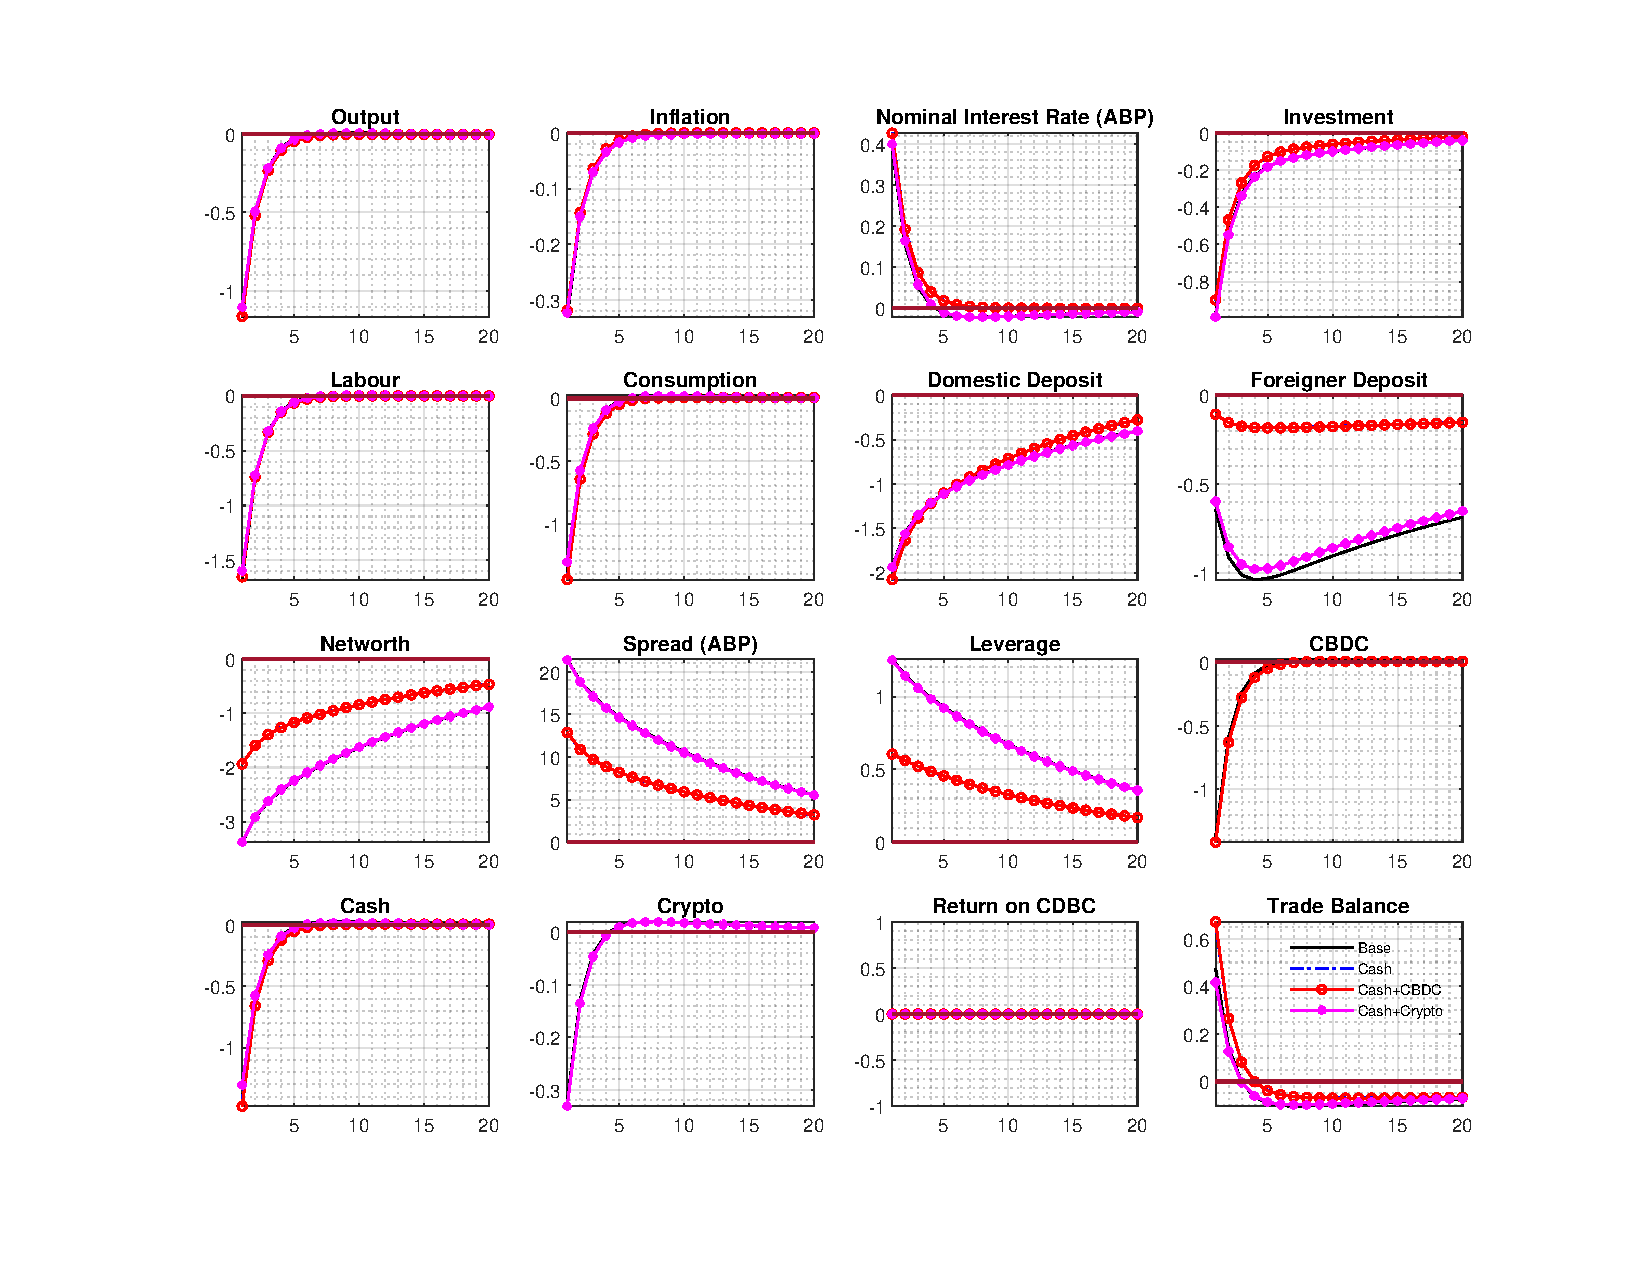
\includegraphics[trim = 0mm 23mm 0mm 18mm, clip, scale=0.97]{monetary_cashvs.pdf}}
	\caption{Response of selected variables to a 25 basic point contractionary monetary policy shock in the domestic economy. All variables are expressed in percentage deviation from steady state.}
	\label{money}
\end{figure}


Similar to the TFP shock, responses in the banking sector are stronger for a model with cryptocurrency which can be mainly traced back to the decrease in foreign debt. The availability of cryptocurrency financing brings in the substitution effect on sources of funding for banks. As we assume that cryptocurrency is affected indirectly by monetary policy, the substitution effect kicks in because the effect of an interest rate hike is higher for foreign debt with the reaction of the exchange rate. Overall, the model shows that there are no big differences in the introduction of CBDC in the domestic economy. However, allowing cryptocurrency as a type of deposit creates substitution effects among sources of funding for the banking sector. From our model predictions, we see that cryptocurrency may amplify the responses of banking sectors. Therefore, it gives rise to concern about regulating cryptocurrency in the financial sector.

Finally, following strong empirical evidence on the "Global Financial Cycle" by \cite{miranda2020us}, \cite{miranda2020global}, the foreign monetary shocks are particularly important for emerging markets and developing countries because the financial markets became progressively more integrated internationally over the past decades. Moreover, due to post-Covid high inflation all around the world, central banks have begun their race on raising the monetary rate. This imposes a great challenge for emerging markets. Hence, we will look at our model responses to the increase in foreign (global) interest rates.

Now, we consider a 25 basic point shock of foreign interest rate. First, the shock cause contraction in the domestic output. As the domestic currency loses its attraction, the real exchange rate depreciates by around 2\%. The real exchange rate depreciation boosts export mostly through an expenditure-switching effect because of the positive price elasticity of export demand. This should sustain the output by the aggregate demand. However, the depreciation in the exchange rate raises the inflation rate by increasing the price of imported goods. The central bank reacts to inflationary pressure and exchange rate stabilisation by raising the interest rate by around 0.6\% annually. Consumption drops follow the increase in the saving rate. Even though the high inflation environment helps to reduce the real burden of home-currency-denominated debt, the fall in asset price followed by an interest rate hike and increase in foreign debt followed by real exchange rate depreciation decrease net worth significantly. The increase in credit spread follows as a consequence to compensate for a higher-risk financial market. Hence, the investment decreases dramatically after the shock following the shrinkage in demand in production sectors. The relationship between worsening bank balance sheet and falls in investment and capital price is similar to \cite{kiyotaki1997credit} and \cite{gertler2015monetary}. Including the foreign borrowing with foreign currency denominated magnifies the effects following \cite{aoki2016monetary}. As these contractionary effects through the bank's balance sheet dominate an expansionary effect of export stimulus in our small open economy. CBDC and cash drop followed by a decrease in demand for consumption goods.


\begin{figure}[H]
  \hspace{-0.7cm}
	\centering
	\centerline{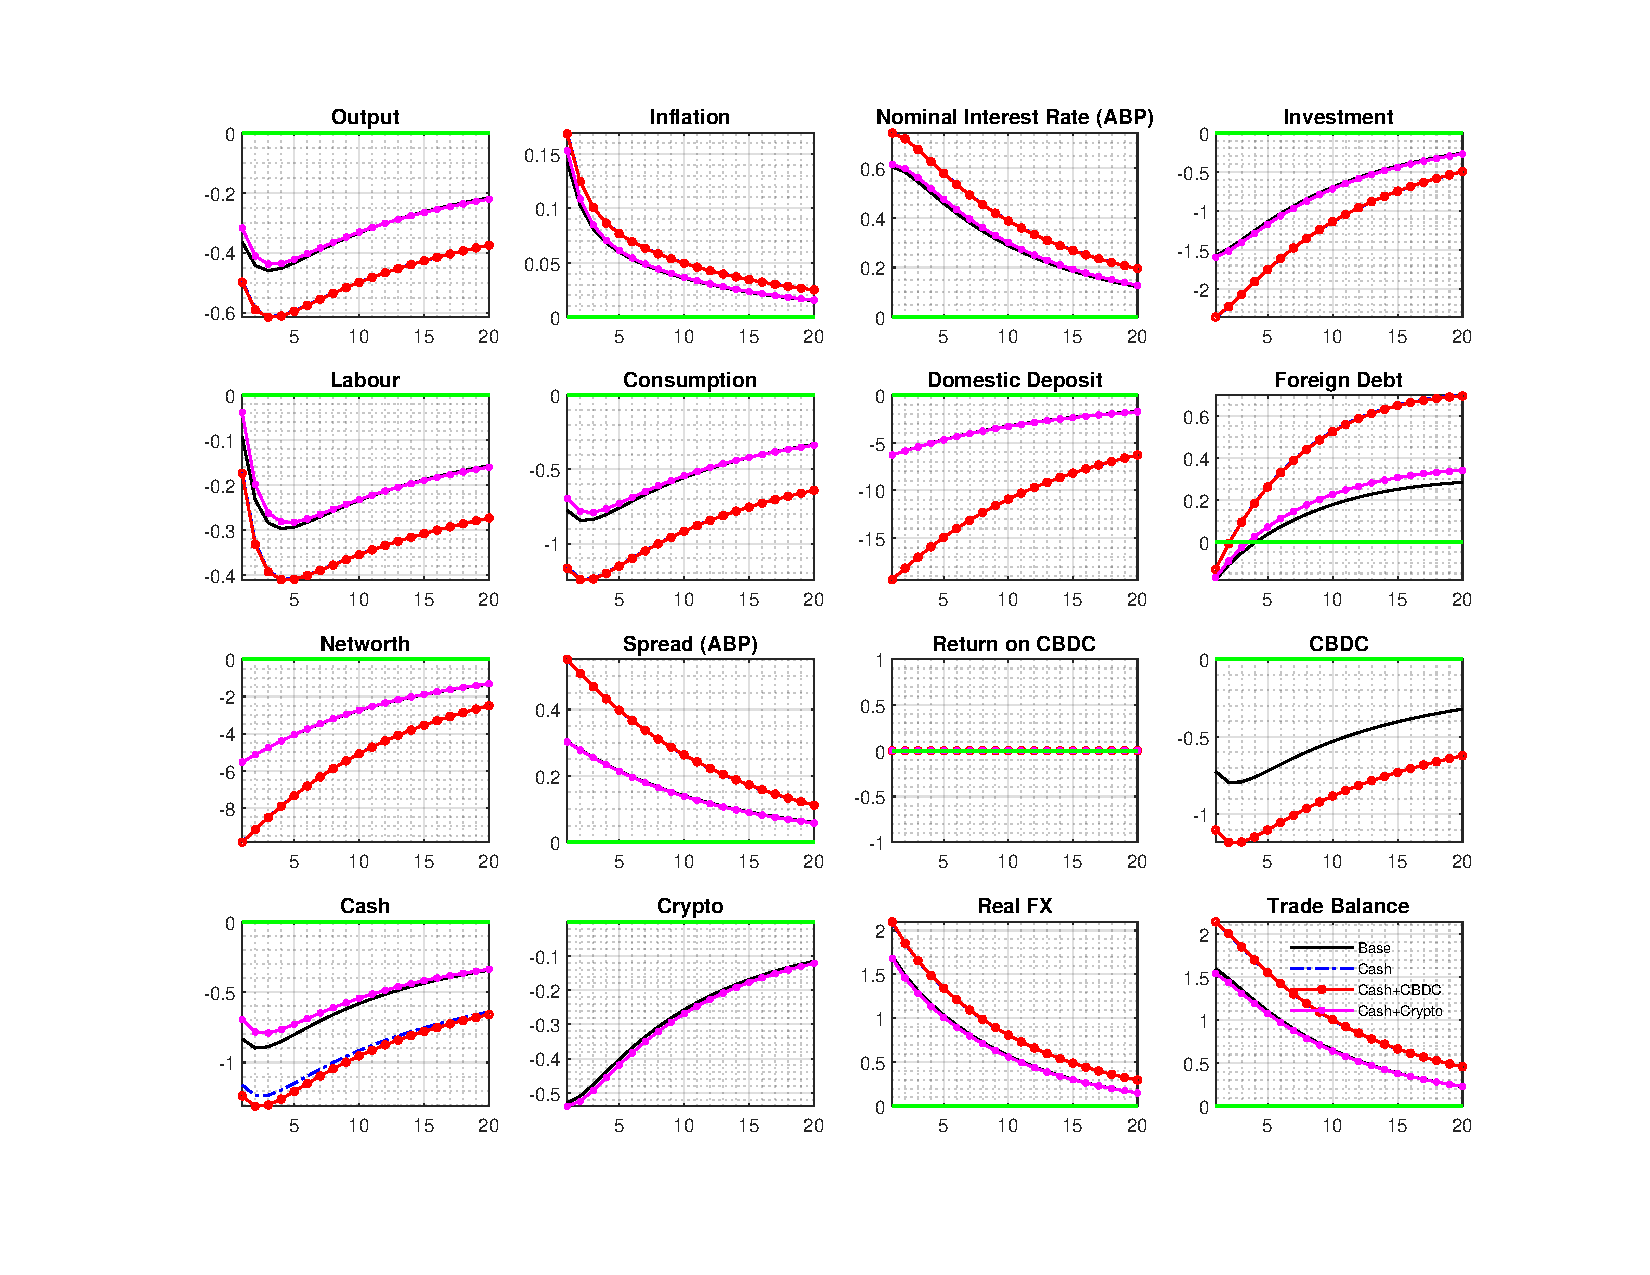
\includegraphics[trim = 0mm 23mm 0mm 18mm, clip, scale=0.97]{foreign_cashvs.pdf}}
	\caption{Response of selected variables to a 25 basic point contractionary foreign monetary policy shock in the domestic economy. All variables are expressed in percentage deviation from steady state.}
	\label{foreign}
\end{figure}


Having been studied for a long time, an emerging market economy is highly vulnerable to the foreign borrowing interest rate hike because it leads to a "debt deflation". This kind of inflation raises the value of foreign currency-denominated debt through exchange rate depreciation and a "credit cycle" of falling productive asset values: both depress the aggregate investment and production through the worsening of the balance sheet of intermediaries (\cite{aoki2016monetary}).

The foreign interest rate shock reveals some interesting points on incorporating cryptocurrencies and CBDC inside an emerging market macroeconomic model. First, the presence of cryptocurrency in the banking sector reduces the effect of foreign rate shock significantly. This is mainly due to the substitution effects on funding sources for the banking sectors. As the domestic interest rate adjusts with inflation and the exchange rate, the funding cost from domestic agents increases. Without an additional option of cryptocurrency funding, bankers suffer more from increasing funding costs domestic and abroad. As can be seen from Figure \ref{foreign}, the presence of cryptocurrency helps to mitigate the transmission of the shock with a smaller change in net worth, spread and foreign debt. By reducing the need for foreign debt, cryptocurrencies also help to dampen the depreciation of the exchange rate. Thus, the nominal rate reacts less strongly. As a result, output, consumption and investment drop more intensively for the model without cryptocurrency. However, we only consider the case that cryptocurrency holders are not foreigners. This is important to mention due to two reasons. First, the funding cost with cryptocurrency is not subject to exchange rate fluctuation compared to foreign deposits. Second, for foreign interest rate shocks, the foreign holders of cryptocurrencies take into account the increase of lending by cryptocurrencies instead of other forms of investment due to a higher foreign interest rate. Thus, they may ask for a higher return rate for cryptocurrency deposits in other countries.  Lastly, as the reaction in consumption is different among model versions, the changes in CBDC and cash are also different. However, we note that the differences are not highly significant.

With baseline simulation, we note that allowing for cryptocurrency deposits in the banking sector affects the responses of core macroeconomic variables to shocks. We observe many deviations among model versions with foreign interest rate shock which is crucial for emerging markets. This is different from the finding of \cite{murakami2021cryptocurrencies} with separated holders of cryptocurrencies. Also, the model assumes high elasticity for cryptocurrency for households due to low liquidity ability. This is crucial to depict the fact that cryptocurrency is not prefered to be a payment instrument but rather for investment purposes.  Also, we observe that implementing CBDC does not come with significant changes in core macroeconomic variables in response to shock. This is in line with the results of \cite{minesso2022central} who find that the effect on the domestic economy is rather negligible but implementing CBDC has a significant effect on the international market. However, we use the Base model in which CBDC have a fixed return. Hence, the difference between cash and CBDC in the base model is minimal. In the next section, we will see the implications of alternative designs on CBDC.


\subsection{Results of alternative CBDC designs}
In this section, I present the results of alternative CBDC designs. We investigate the implications of CBDC through three kinds of shocks and four different designs of CBDC. The Base model means a fixed return on CBDC holding. The Flex model means that the return of CBDC follows a Taylor rule which makes it compatible with deposits. The Markdown model means that the return of CBDC reacts with a constant spread to the nominal rate. Lastly, the Quantity model means that the amount of CBDC is a fixed proportion of GDP and the return is determined by the market. 
\begin{align*}
    &\textbf{Flex model:}\quad \left(\frac{{{R}_{t}^{DC}}}{{\bar R^{DC}}}\right)=  \left(\frac{{{R}_{t-1}^{DC}}}{{\bar R^{DC}}}\right)^{\rho_{rdc}} \left(\left(\frac{\pi_t}{\bar \pi}\right)^{\phi^{\pi_dc}} \left(\frac{Y_t}{Y}\right)^{\phi^y}\right)^{1-\rho_{rdc}}\\ 
     &\textbf{Markdown model:} \quad {R}_{t}^{DC}=R_t -{R}_{spread}^{DC} \\
     & \textbf{Quantity model:} \quad DC_t^{supply} = \Upsilon Y_t, \quad DC_t^{supply} = P_t^{DC} DC_t , \quad {R}_{t}^{DC} = \frac{P_t^{DC}}{P_{t-1}^{DC}}
\end{align*}



\begin{figure}[H]
  \hspace{-0.7cm}
	\centering
	\centerline{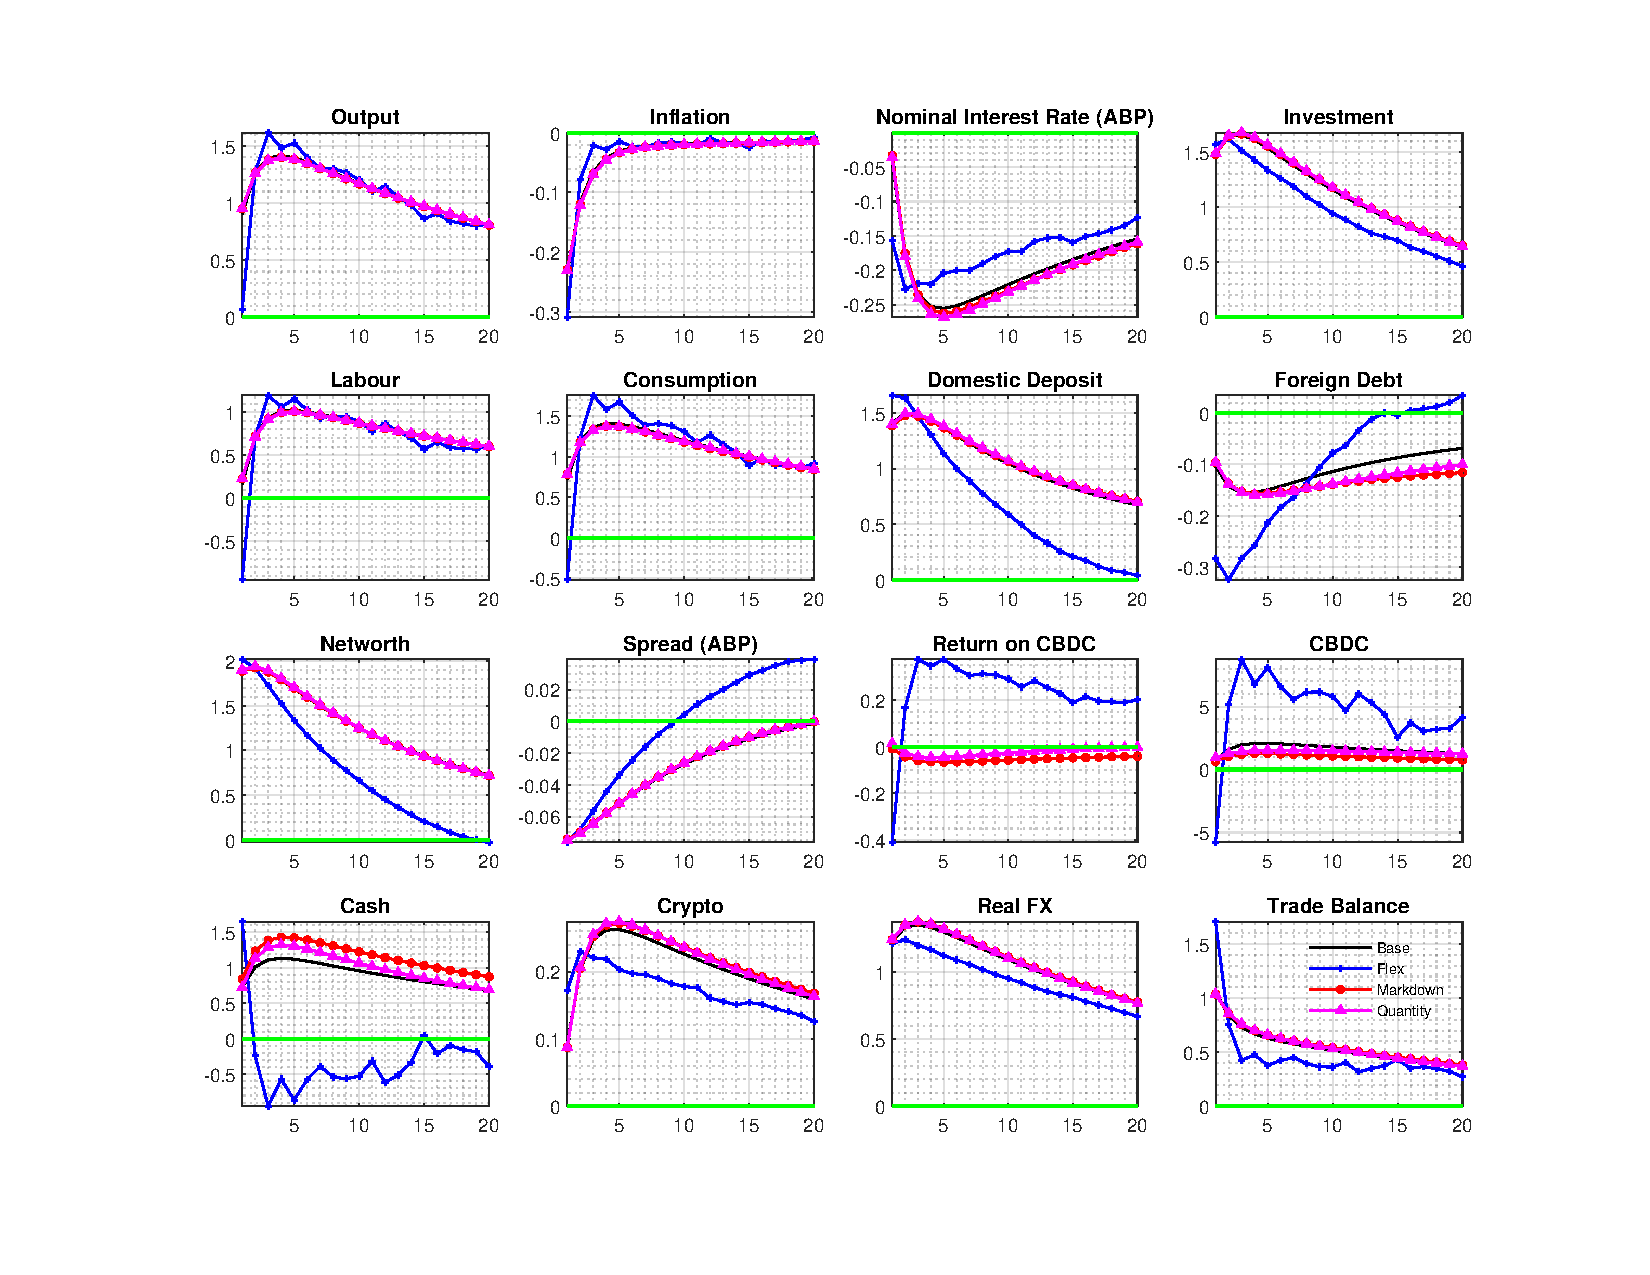
\includegraphics[trim = 0mm 23mm 0mm 18mm, clip, scale=0.97]{TFP_alt.pdf}}
	\caption{Response of selected variables to a one standard deviation expansionary total factor productivity shock in the domestic economy. All variables are expressed in percentage deviation from steady state.}
	\label{TFPalt}
\end{figure}

Again, we look at the impulse response functions of three main shocks. As pointed out from the beginning, CBDC is a hybrid instrument which can be used for payment and saving at the same time. Allowing for different designs on CBDC, the model predicts significant differences in responses of the economy. Using a Taylor-type rule for return rate on CBDC, we see that the Flex model differs the most from the other models. For all three shocks, the Flex model shows that the output reacts stronger to shocks compared to the Base model. Besides, the flexible rate on CBDC seems to interact with the responses of the monetary rate. This reaction of output is mainly followed by consumption but not investment because the model implies that only cash and CBDC can be used for payment of consumption. Hence, altering the CBDC design has a direct effect on consumption. 

\begin{figure}[H]
  \hspace{-0.7cm}
	\centering
	\centerline{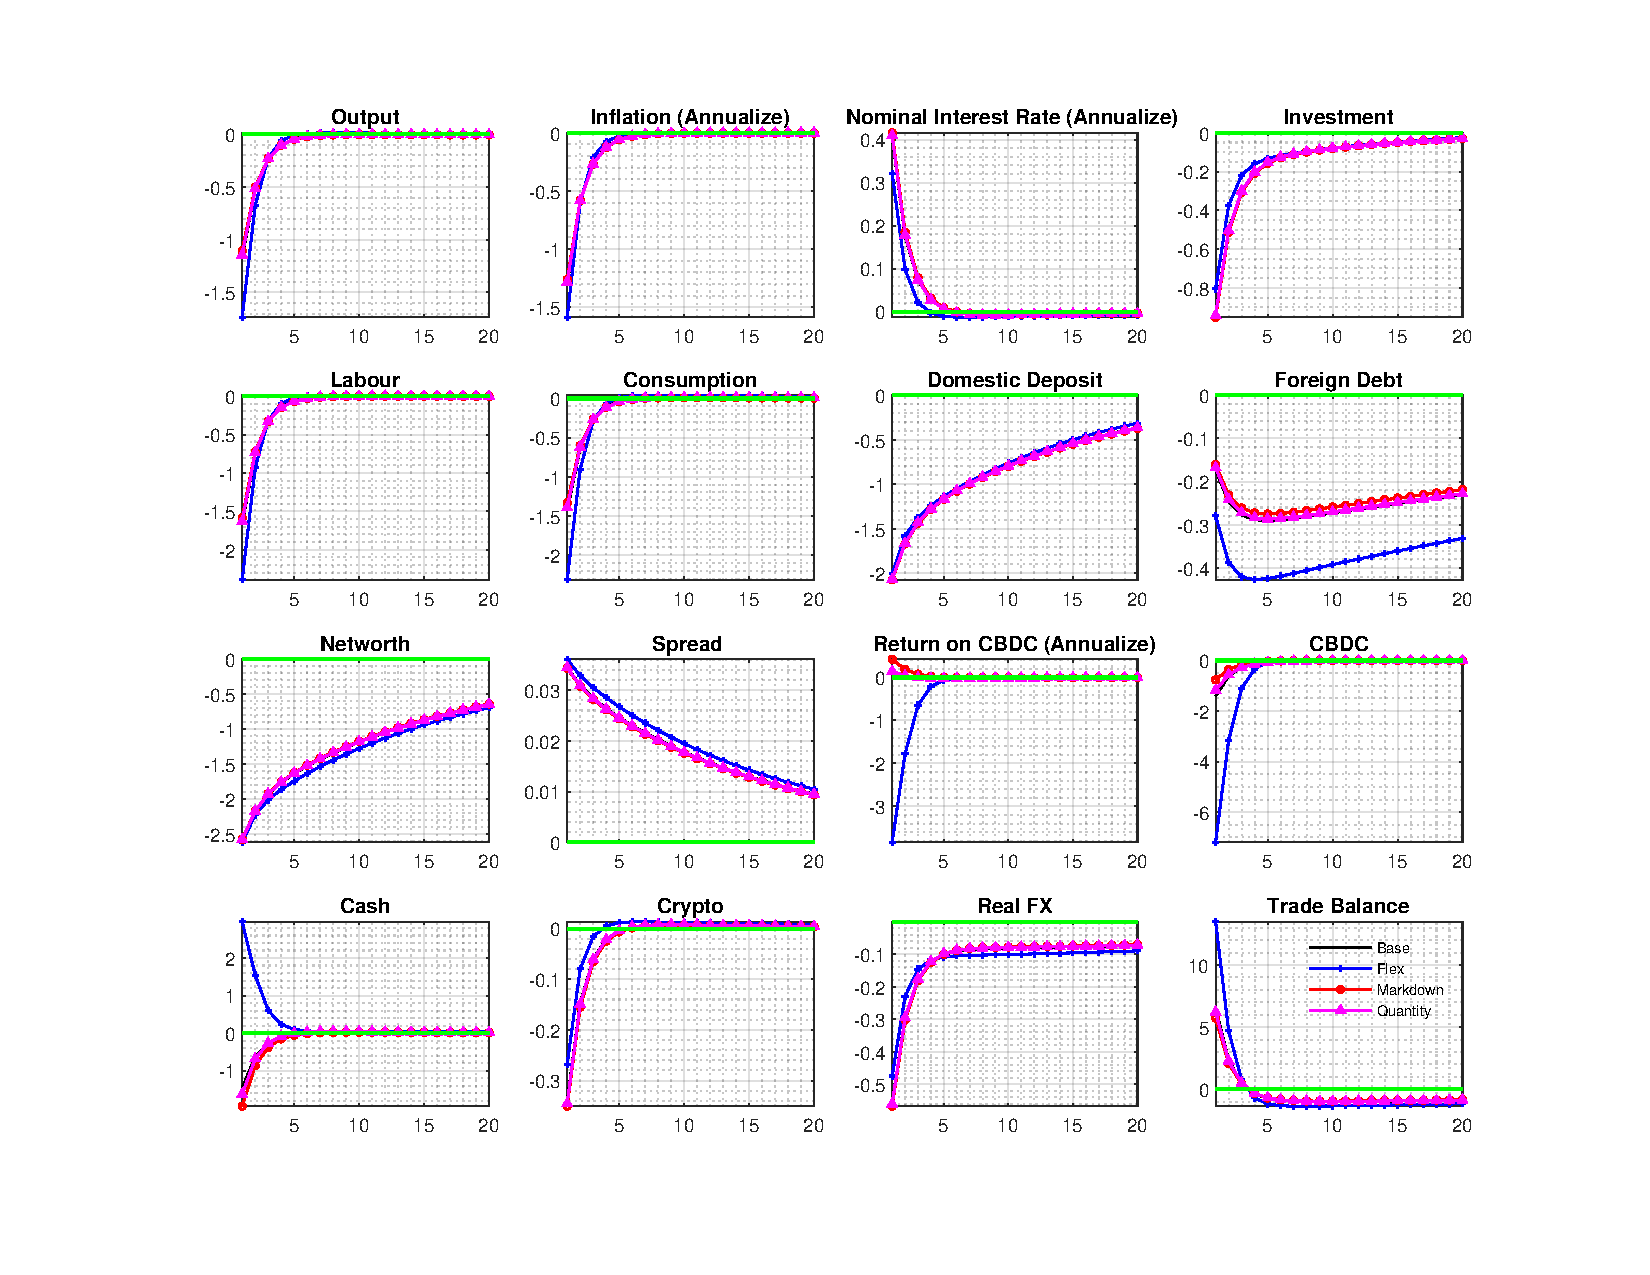
\includegraphics[trim = 0mm 23mm 0mm 18mm, clip, scale=0.97]{monetary_alt.pdf}}
	\caption{Response of selected variables to a 25 basic point tightening monetary policy shock in the domestic economy. All variables are expressed in percentage deviation from steady state.}
	\label{monalt}
\end{figure}

Looking broadly, allowing for flexible return on CBDC also affects other macroeconomic factors. Inflation and investment also react differently compared to the Base model. As inflation seems to react stronger with the flexible rate, investment decrease less in the Flex model with a contractionary domestic monetary shock. This is due to the substitution effect between consumption and investment. Moreover, the nominal interest rate reacts slighter when we allow for the CBDC rate to react to the inflation rate and output. Hence, under the model scope, CBDC flexible rate can also share the work of the nominal rate in fighting inflation. Hence, it reduces the reaction of the nominal interest rate to shocks. This is important for emerging markets as it reduces the pressure on the exchange rate with the changes in nominal rate which plays a crucial role in conducting emerging markets policies. 

Lastly, because CBDC can affect the nominal interest rate, it affects the foreign debt indirectly. This observation comes from the optimization problem in the banking sector where there is a substitution effect between domestic and abroad funding sources. First, it is worth mentioning that the foreign borrowing burden is affected by the foreign interest rate and the fluctuation of the exchange rate. In our case, the exchange rate reacts less forceful following the dynamic of the nominal interest rate. Hence, it reduces the value of foreign debt. Second, the domestic nominal rate decreases more with a TFP shock and increases less with an interest rate shock means a smaller increase in the cost of domestic borrowing. Hence, it helps to decrease the foreign debt in both cases.

\subsection{Optimal monetary policy rule}

In this part, I conduct the optimal welfare policy exercise for the model without CBDC and four alternative designs of CBDC. We want to see the role of CBDC and its designs on optimal policy. To address this question, we now turn to the analysis of the systematic component of monetary policy. Following other literature on optimal policy, I compute the reaction to inflation and depreciation rate parameters of the monetary policy rule that maximizes household welfare. Welfare is defined as a recursive form as $W_t= U_t +E_t \beta W_{t+1} $ in which it is a sum of current and expected future utility. Our model is solved at second-order approximation with the pruning method and the welfare gain is reported under consumption equivalent. The results are shown in Table \ref{optimal}.


\begin{figure}[H]
  \hspace{-0.7cm}
	\centering
	\centerline{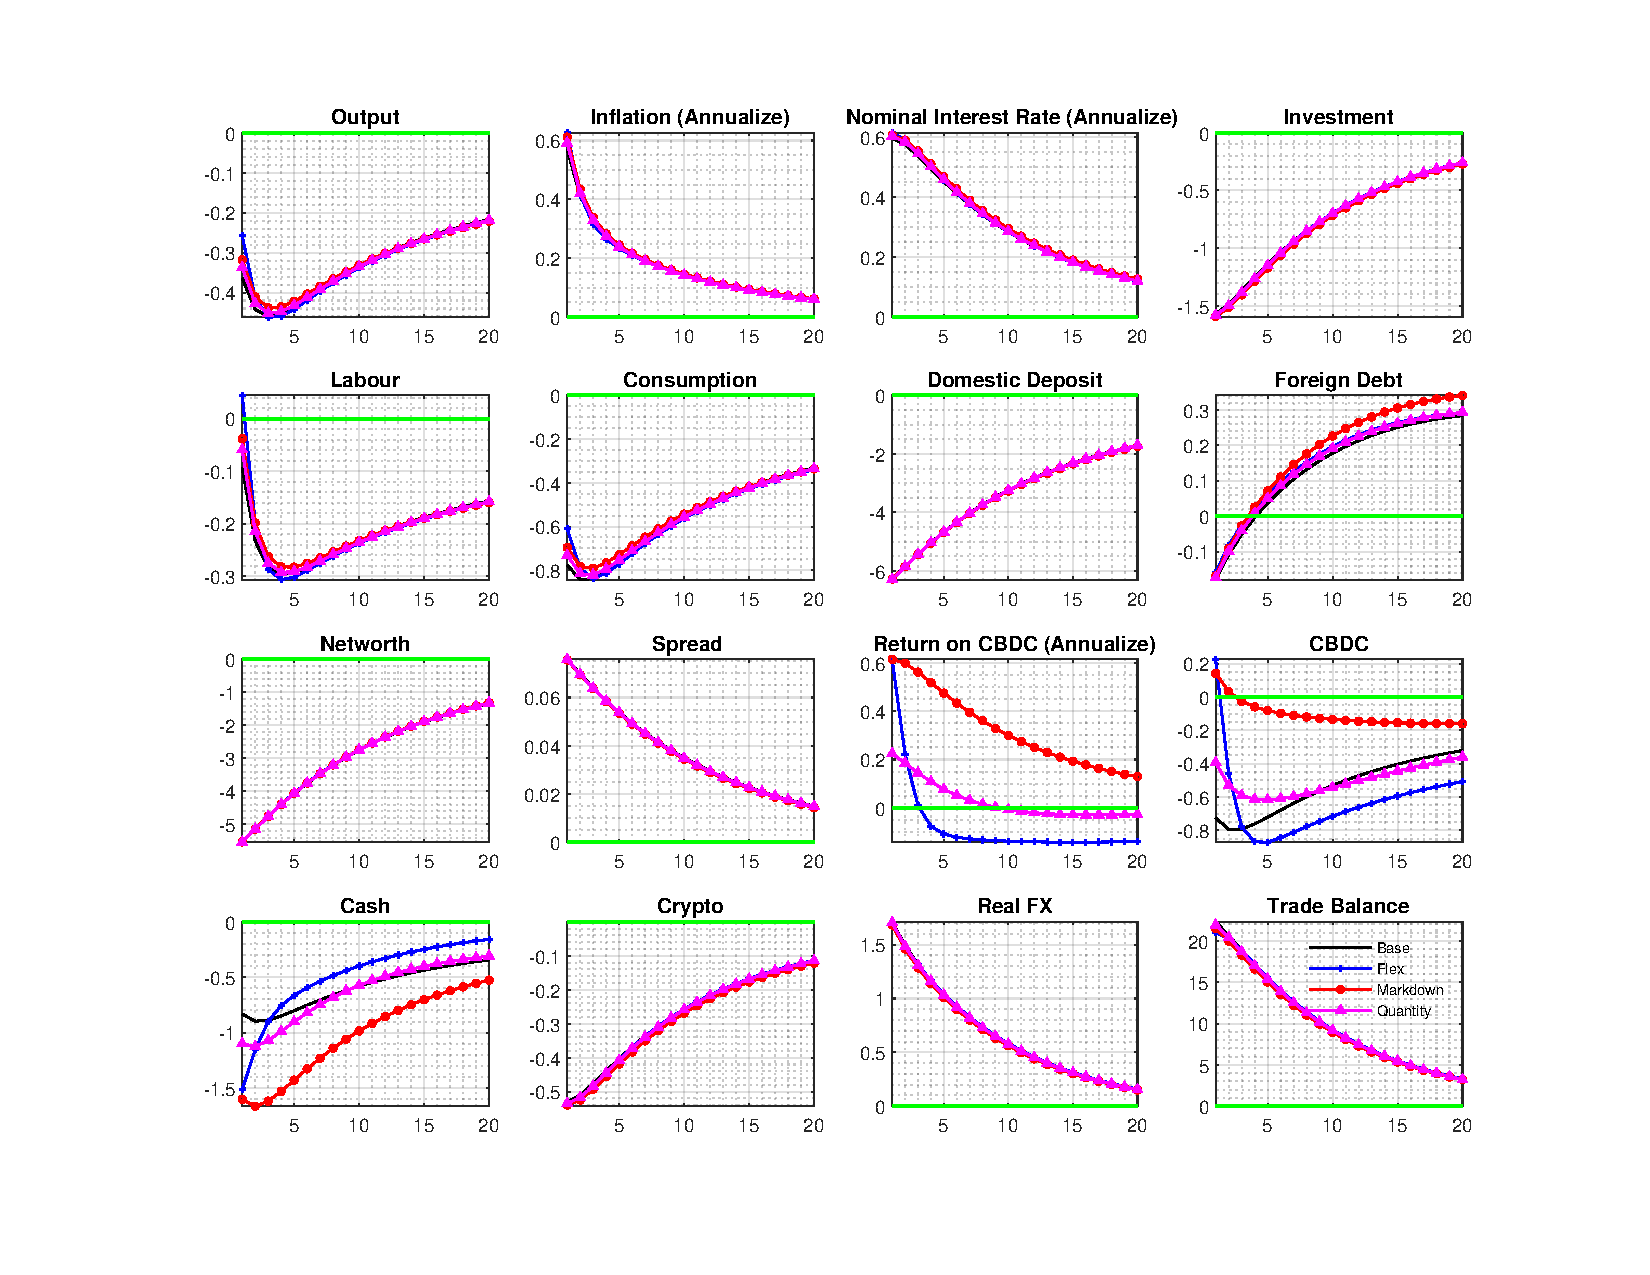
\includegraphics[trim = 0mm 23mm 0mm 18mm, clip, scale=0.97]{foreign_alt.pdf}}
	\caption{Response of selected variables to a one standard deviation expansionary foreign monetary policy shock in the domestic economy. All variables are expressed in percentage deviation from steady state.}
	\label{foralt}
\end{figure}

Different from other optimal welfare exercises on the policy rule, we do not impose an upper bound on the response to inflation. This is a common approach due to price stability can have a big effect on welfare. Except for the Flex version, all others show that they will put all the weight on fighting inflation but not stabilizing the depreciation rate. This finding is in line with \citep{akinci2018exchange} who also conduct a welfare analysis using the exchange rate targeting with the ABK model. \citep{akinci2018exchange} find that there are significant welfare losses with exchange rate targeting in addition to inflation targeting. Notably, the Flex version returns a positive value in response to the depreciation rate. This suggests that implementing the flexible rule on CBDC can provide valuable help to conventional policy on fighting inflation. Thus, it provides space for targeting the depreciation rate which is important for emerging markets.



\begin{table}[H]
\caption{\label{optimal}Volatility and welfare under the optimal monetary rule: foreign interest rate shocks.}

\hspace{-2.6cm}
\small
\begin{tabular}{c|cc|cc|cc|cc|cc}

\hline
\textbf{Parameters} &\multicolumn{2}{c}{Cash+Cryp} &  \multicolumn{2}{c}{Base} & \multicolumn{2}{c}{Flex} & \multicolumn{2}{c}{Quantity}    & \multicolumn{2}{c}{Markdown} \\

 \hline
   &\small{Baseline}  &  \small{Optimal} & \small{Baseline}  & \small{Optimal} & \small{Baseline}  & \small{Optimal}    & \small{Baseline}  &  \small{Optimal} & \small{Baseline}  & \small{Optimal} \\ 
\hline
 $\phi_{\pi}$&   1.49 &  7.5686 & 1.49 & 7.4864   &  1.49 &  5.9683      &      1.49 & 7.6489 &1.49 &  8.0006    \\
 $\phi_e$&  0.3 & 0 & 0.3 &  0  &0.3   &  0.0886      &     0.3 & 0    &     0.3  &       0 \\        
 \hline

 \textbf{Volatility} & \\
 \hline
Output 	 & 2.1157  & 2.2915 & 2.1186 &  2.2853 &   2.1099   &  2.2780 &       2.1139  &  2.2874 & 2.1157 &   2.2950 \\
Consumption & 3.5352 &   3.7010 & 3.5849  &  3.7204	 & 	3.5686  &  3.7531 &  3.5692  &  3.7136   & 3.5354  & 3.7052  \\
Inflation & 0.2800 &   0.0569  & 0.2675   & 0.0569 &   0.2737 &   0.0622      &        0.2721  &  0.0575  &0.2800  &  0.0540 \\
Net-worth & 17.5905 &  19.4314 & 17.6745  & 19.3794 &	   17.6270 &  19.4142 & 17.6475  & 19.4480 & 17.5903 &  19.4743\\
CBDC &N/A & N/A&  3.4458  & 3.6350 &	 3.0215  &  1.1414 &     3.2764   &  3.4603 & 1.5629  &  2.4154\\
Crypto &  1.6137  &   1.0443 & 1.5552 &   1.0154 &	 4.6945  &  6.3762     &      1.5702  &  1.0344 & 1.6135 &   1.0421\\
Cash	 &  3.5352   & 3.7010 &  3.7364   &  3.8130 & 	1.5618  &  1.0255     &       3.9870  &   4.0798 & 6.0611 &   5.1795\\
Foreign Debt & 3.9377  &   3.5764 & 3.5423  & 3.3685 & 	  3.4456 &   2.9292     &   3.5887  &  3.3929 & 3.9370  &  3.5672 \\
\hline
\textbf{Welfare gain} &  \\
\hline
$\Delta$ W\tablefootnote{Consumption equivalence to steady state welfare} & 1.3525\% &   1.4040\% & 1.3615\% &   1.4056\% & 1.3423\%  &  1.3860\% & 1.3560\%  & 1.4017\% &  1.3450\%  &  1.4016\%

\end{tabular}
\end{table}



\section{Conclusion}
This paper studies the implications of CBDC inside an emerging market economy with cryptocurrency. We build an open economy model with CBDC, cryptocurrency inside the banking sector with foreign debt. The results of this paper shed some light on a growing body of literature on digital assets, CBDC, and the digital economy. Some of these results are in line with the existing literature. In particular, I also find that the introduction does not affect the domestic macroeconomic variables significantly when the return on CBDC is fixed as 1. With the fixed return of CBDC as 1, we assume that CBDC is only used for payment but not for saving. However, different from the results of \cite{murakami2021cryptocurrencies}, I find that allowing bankers to hold cryptocurrencies as a source of funding can mitigate the negative effect of some shocks. The reason is due to the fact that the return of cryptocurrency is partly shielded from changes in the domestic and abroad policy rate. Hence, this allows the banking sector to have more options for funding sources. The main reason can be traced back to the fact that I implement a different form of the utility function and assume the household can hold cash, CBDC and cryptocurrency at the same time compared to \cite{murakami2021cryptocurrencies}. This gives rise to a substitution effect for households in responding to shocks. Surprisingly, with CBDC and cryptocurrencies, we observe significant changes in the dynamic of foreign debt. Cryptocurrency and CBDC seem to help reduce the dependence on foreign debt which is important for an emerging market economy. However, the model is not able to depict the high volatility of cryptocurrency. Moving forward, alternative designs of CBDC reveal many more interesting observations. I find that CBDC can provide an additional tool for central banks and support the nominal rate in achieving the central bank's targets. Last but not least, a flexible rate in CBDC return can also affect the responses in the banking sector. To the best of my knowledge, there is yet a model to include CBDC and cryptocurrency for an emerging market model with financial frictions.

Nevertheless, this model has not included some relevant features of CBDC in an emerging market which should be tackled in future. First, for instance, we do not include the possibility of firms either using foreign capital (i.e foreign direct investment firms) or borrowing directly from abroad (i.e foreign currency or foreign CBDC). Second, we can allow the banking sectors to hold CBDC as a reserve requirement. Third, I have not implemented any macroprudential policy on either domestic or abroad borrowing. Hence, the question about the interaction of CBDC and macroprudential tax has remained doubtful. Last but not least, the possibility for households to hold foreign CBDC such as the Digital Dollar is crucial to study in the sense of optimal capital flow management for emerging markets policymakers. Allowing domestic households to trade foreign CBDC will affect the USD reserve of the central bank. Hence, it limits the power of emerging market central banks to conduct foreign exchange intervention policy to stabilise the domestic economy from foreign shocks such as exchange rates or foreign interest rate shocks. Although our model has already shed some light on the effect of foreign interest rate shock, including all the above features might change the results significantly. Finally, results are generated with our model structure and assumptions as well as our parameterisation. Hence, using the model for policy need to be conducted with caution and estimation of the model is highly desired with a specific dataset. These issues are left for future research.

\newpage

\bibliography{cbdc}
\bibliographystyle{aea}
\newpage
\appendix
\numberwithin{equation}{section} %restarts equation numbering with 1 and adds the appendix in front
\numberwithin{table}{section} %same for Tables
\numberwithin{figure}{section} %and for Figures

\section{Appendix 1: Details on derivations}
%\footnote{For more detailed derivations, viewer can read \cite{aoki2016monetary}}
\subsection{Households}
\begin{align}
   U_t=  E_t \sum_{t=0}^{\infty} \beta^t\left[ ln\left(C_t-\zeta_{0}\frac{H_t^{1+\zeta}}{1+\zeta}\right) -\chi_{DC}\varrho\left(\frac{M_t}{M_t+DC_t},\Gamma\right) +\mu^C\left(\frac{Cryp_t}{1-\sigma^c}\right)^{1-\sigma^c}\right] 
\end{align}
\begin{align*}
&\text{s.t.}  \nonumber\\
  & C_t + D_{t} + B_t + Q_t K^h_t  + M_t + DC_t + Cryp_t +\chi^h(K^h_t,K_t) \\   
 & = w_t H_t + \frac{R_{t-1}}{\pi_t} B_{t-1}+ \frac{R^D_{t-1}}{\pi_t} D_{t-1} + (Z_t+ \lambda Q_t) K^h_{t-1} + \epsilon^m M_{t-1} + \frac{R^{DC}_{t-1}}{\pi_t} DC_{t-1} +\frac{R^{C}_{t-1}}{\pi_t} Cryp_{t-1}  +\Pi_t 
\end{align*}

We assume that consumption goods are only paid by cash and CBDC. Thus, the cash in advance is following:
\begin{align}
    C_t=[\mu^m M_t^{1-\rho_{dc}} + \mu^{DC}DC_t^{1-\rho_{dc}}]^{\frac{1}{1-\rho_{dc}}}
\end{align}
The re-balancing utility loss function takes the following functional form:
\begin{align}
    \varrho\left(\frac{M_t}{M_t+DC_t},\Gamma\right)= \left(\Gamma-\frac{M_t}{M_t+DC_t} \right)^2
\end{align}
\subsection{Bankers}
Similar to \cite{aoki2016monetary} and \cite{gertler2011model}, we write the banker's problem in a recursive form:
\begin{align}
V_t(N_t)= \max_{K^b_t, D_t, D^*_t} E_{t}\Lambda_{t;t+1}[ (1-\sigma)N_{t+1}+\sigma V_{t+1}(N_{t+1})]
\end{align}
Rewritten in term of Tobin's Q as:
\begin{align}
  \psi_t=  \frac{V_t}{N_t} = E_{t}\Lambda_{t;t+1}[ (1-\sigma)+\sigma \varkappa_{t+1}\left(\frac{N_{t+1}}{N_{t}}\right)]
\end{align}
Including the flow of fund, we rewrite:
\begin{align}
    \frac{N_{t+1}}{N_{t}}= \frac{Z_{t+1}+Q\lambda_{t+1}}{Q_t}lev_t-\frac{{R}_{t}}{{\Pi}_{t+1}}-\frac{{s_t D^{*}}_{t}{R^{*}}_{t}}{\Pi^*_{t+1}} -\frac{ {Cryp}_{t}\, {R^c}_{t}}{{\Pi}_{t+1}}
\end{align}
As we assume amount of cryptocurrency and foreigner deposit relate to leverage as $\frac{s_t D^{*}_{t}}{n_{t}}=x_t lev_t$ and  $\frac{{ Cryp_t}_{t}}{n_{t}}=x^c_t lev_t$, we have definition for $\frac{ D_{t}}{n_{t}}$ as:
\begin{align}
    \frac{D_{t}}{n_{t}} =  \left(1+\frac{\varkappa_{b}}{2} x^2_t\right) lev_t - x_t lev_t  -x^c_t lev_t
\end{align}
Then we express Tobin's Q as:

\begin{align}
 \psi_t=  \mu_t lev_t + \left(1+\frac{\varkappa_{b}}{2} x^2_t lev_t \right) lev_t +\mu^* x_t lev_t +\mu^c x^c_t lev_t
\end{align} 

Now, we can rewrite the banker optimization problem into the Lagrangian similar to \cite{aoki2016monetary} using all the definitions from (21)-(25):

\begin{align}
    \mathcal{L_t} =(1+\lambda_t)\left[\mu_t lev_t +\mu^c_t x^c_t lev_t + \mu^*_t x_t lev_t +\left(1+\frac{\varkappa_{b}}{2} x^2_t\right)v_t \right] -\lambda_t\theta lev_t
\end{align}

Using FOCs, we express a closed form of the fraction of assets funded by foreign borrowing.
\begin{align}
    x_t= \frac{\theta \mu^*_t -\varkappa_{b} v_t }{\theta \varkappa_{b} v_t} +\sqrt{\left(\frac{\mu^*_t}{\varkappa_{b} v_t}\right)^2 +2(\frac{\mu^c_t}{\varkappa_{b} v_t} x^c_t +\left(\frac{1}{\theta}\right)^2 +2\frac{\mu_t}{\varkappa_{b} v_t}}
\end{align}
\subsection{Cryptocurrency producer}
In this part, for modelling cryptocurrency producers (miners), we follow the idea of \cite{asimakopoulos2019new} for including cryptocurrencies from \cite{sockin2018model} into a general equilibrium set-up. As standard, we assume that there is a continuum of cryptocurrency producers indexed by n, where $n \in [0, 1]$, and all miners operate under perfect competition. Similar to \cite{sockin2018model}, producing the number of tokens requires some cost to ensure unlimited supply. The cost of producing relates to the common component and programming skills. Producers conduct their profit maximization as follows:

\begin{align}
\Pi^c_t = \max_{Cryp_t} \left((1-\rho^c)P^c_t -\kappa^{-\varpi_t}\right) Cryp_t  
\end{align}
where $\varpi_t$ governs the efficiency of producers and $ 1-\rho^c$ is  a fraction of revenue from selling to households. The setup is mainly aimed to create a proxy for cryptocurrency producer productivity shock.
\section{Appendix 2: Further Results}
\textbf{Different Storage Cost of Cash:} In this part, I present the results with higher storage of physical cash. This reduces the incentive for households to hold physical cash relative to CBDC. To this extent, even with fixed returns on CBDC, holding physical cash is less preferred compared to holding CBDC. In \ref{TFP_sto}, the smaller value of $\epsilon^m$ means a higher cost of storage of cash compared to CBDC. $\epsilon^m = 0.8$ means a 20\% storage cost while $\epsilon^m = 0.8$ means a zero storage cost. In Figure \ref{TFP_sto}, I report the response of output and CBDC holdings for a positive total factor productivity shock in the domestic economy. The intuition for the results is simple. Higher storage costs make CBDC more attractive relative to cash even without the saving feature for CBDC. It provokes the usage of CBDC compared to cash. Under the flexible rate regime of CBDC, storage cost has a significant effect on the arbitrage condition that links together deposit return, the exchange rate and the interest rate on CBDC. Hence, the effect spreads to consumption and the banking sector which also affects foreign debts.

\textbf{Different Liquidity Level:} In this part, we vary the substitutability between CBDC and cash for the liquidity aggregator in the utility function. Undoubtedly, higher substitutability affects the decisions of households on cash and CBDC in response to shocks. Unlike results for differing storage costs, the difference among different values is not large even though we observe some differences in the dynamic of foreign debt under the flexible return regime of CBDC. Hence, the changes in substitutability between CBDC and cash seem to not change significantly in the general equilibrium of our model.


\textbf{Variance Decomposition:} Lastly, I provide the variance decomposition of three main shocks for 4 different versions of our model. Including cryptocurrency and CBDC in the model increases the effect of TFP shock and decreases the foreign interest rate shock on consumption. Moreover, we observe less volatility in foreign debt in response to a foreign interest rate shock in the model with CDBC and crypto. However, domestic policy rate shock accounts for a bigger role under this circumstance. Hence, including CBDC seems to increase the transmission of domestic monetary policy.

\section{Appendix 3: Figures}
\begin{figure}[H]
    \hspace{-0.1cm}
	\centering
	\centerline{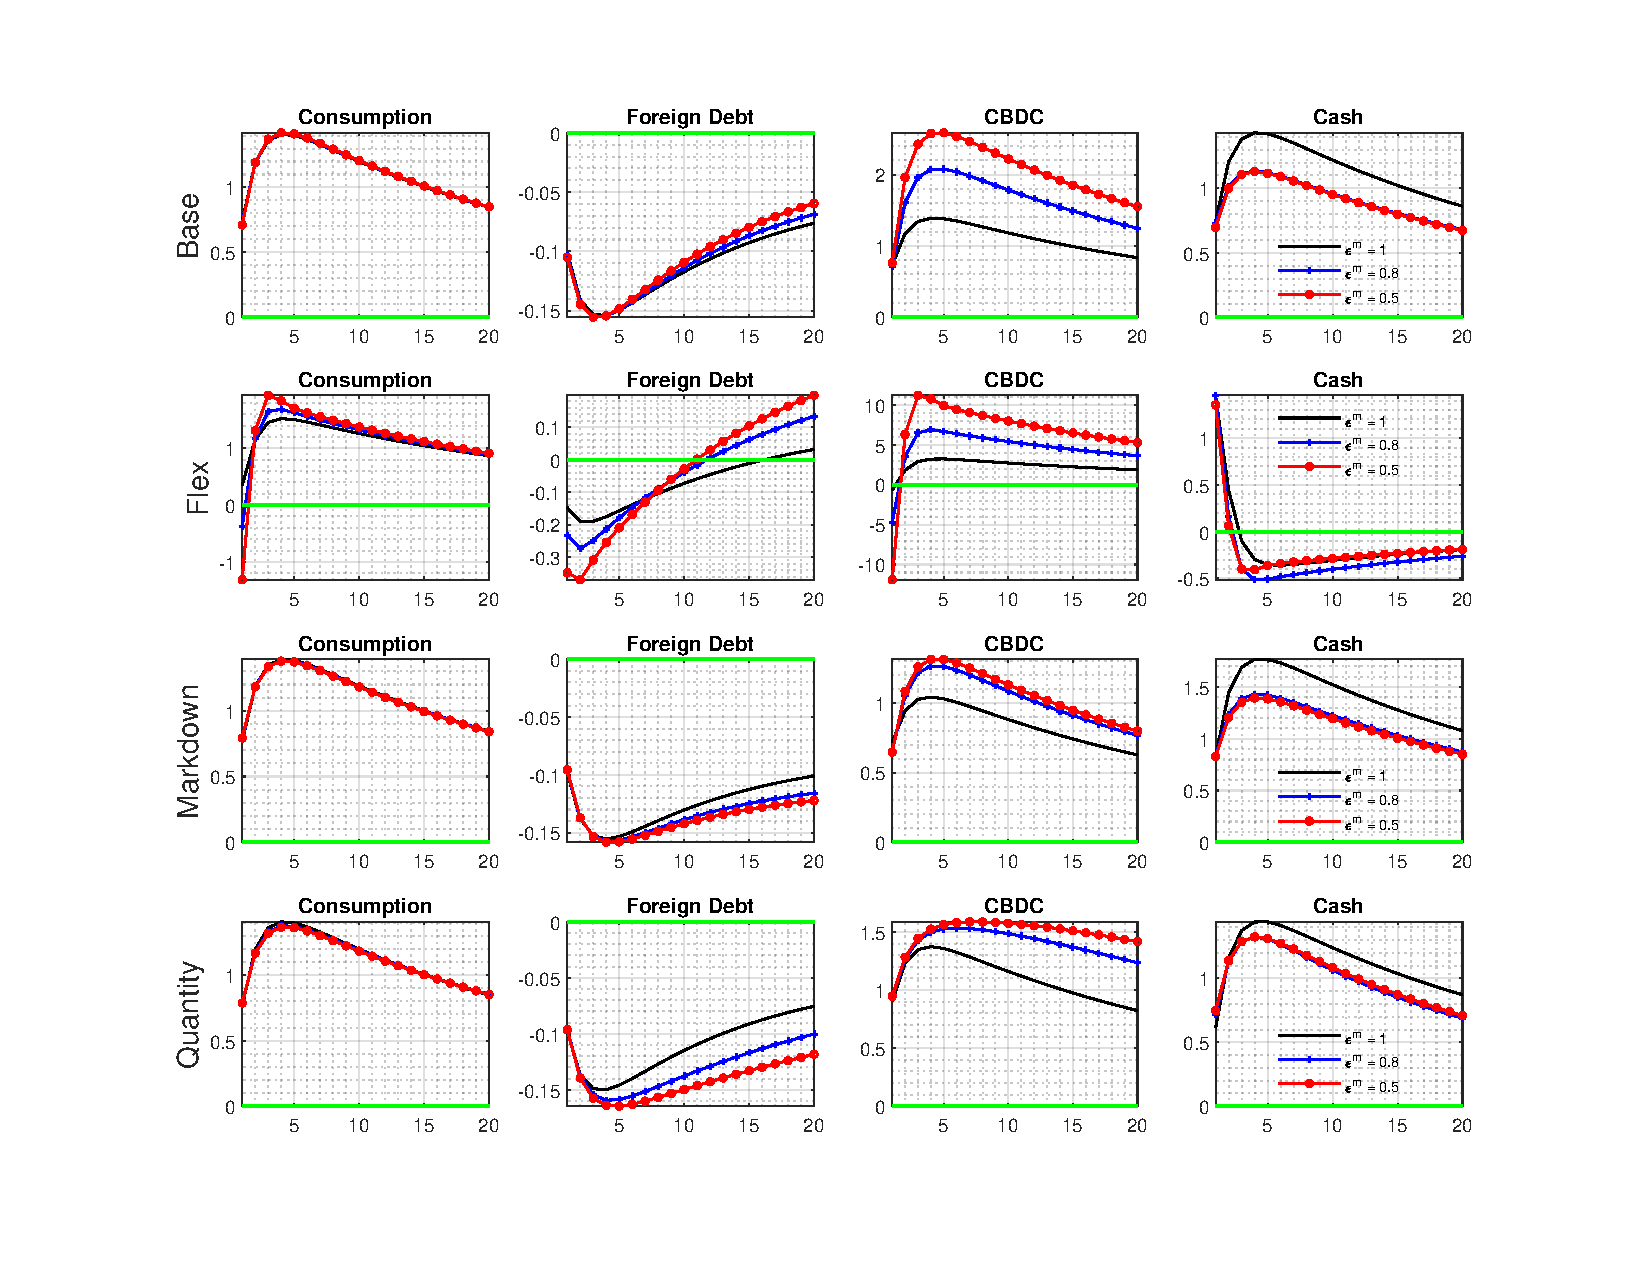
\includegraphics[trim = 0mm 23mm 0mm 18mm, clip, scale=0.93]{TFP_sto.pdf}}
	\caption{Response of selected variables to a 1\% expansionary total factor productivity shock in the domestic economy. All variables are expressed in percentage deviation from steady state.}
	\label{TFP_sto}
\end{figure}
\begin{figure}[H]
  \hspace{-0.1cm}
	\centering
	\centerline{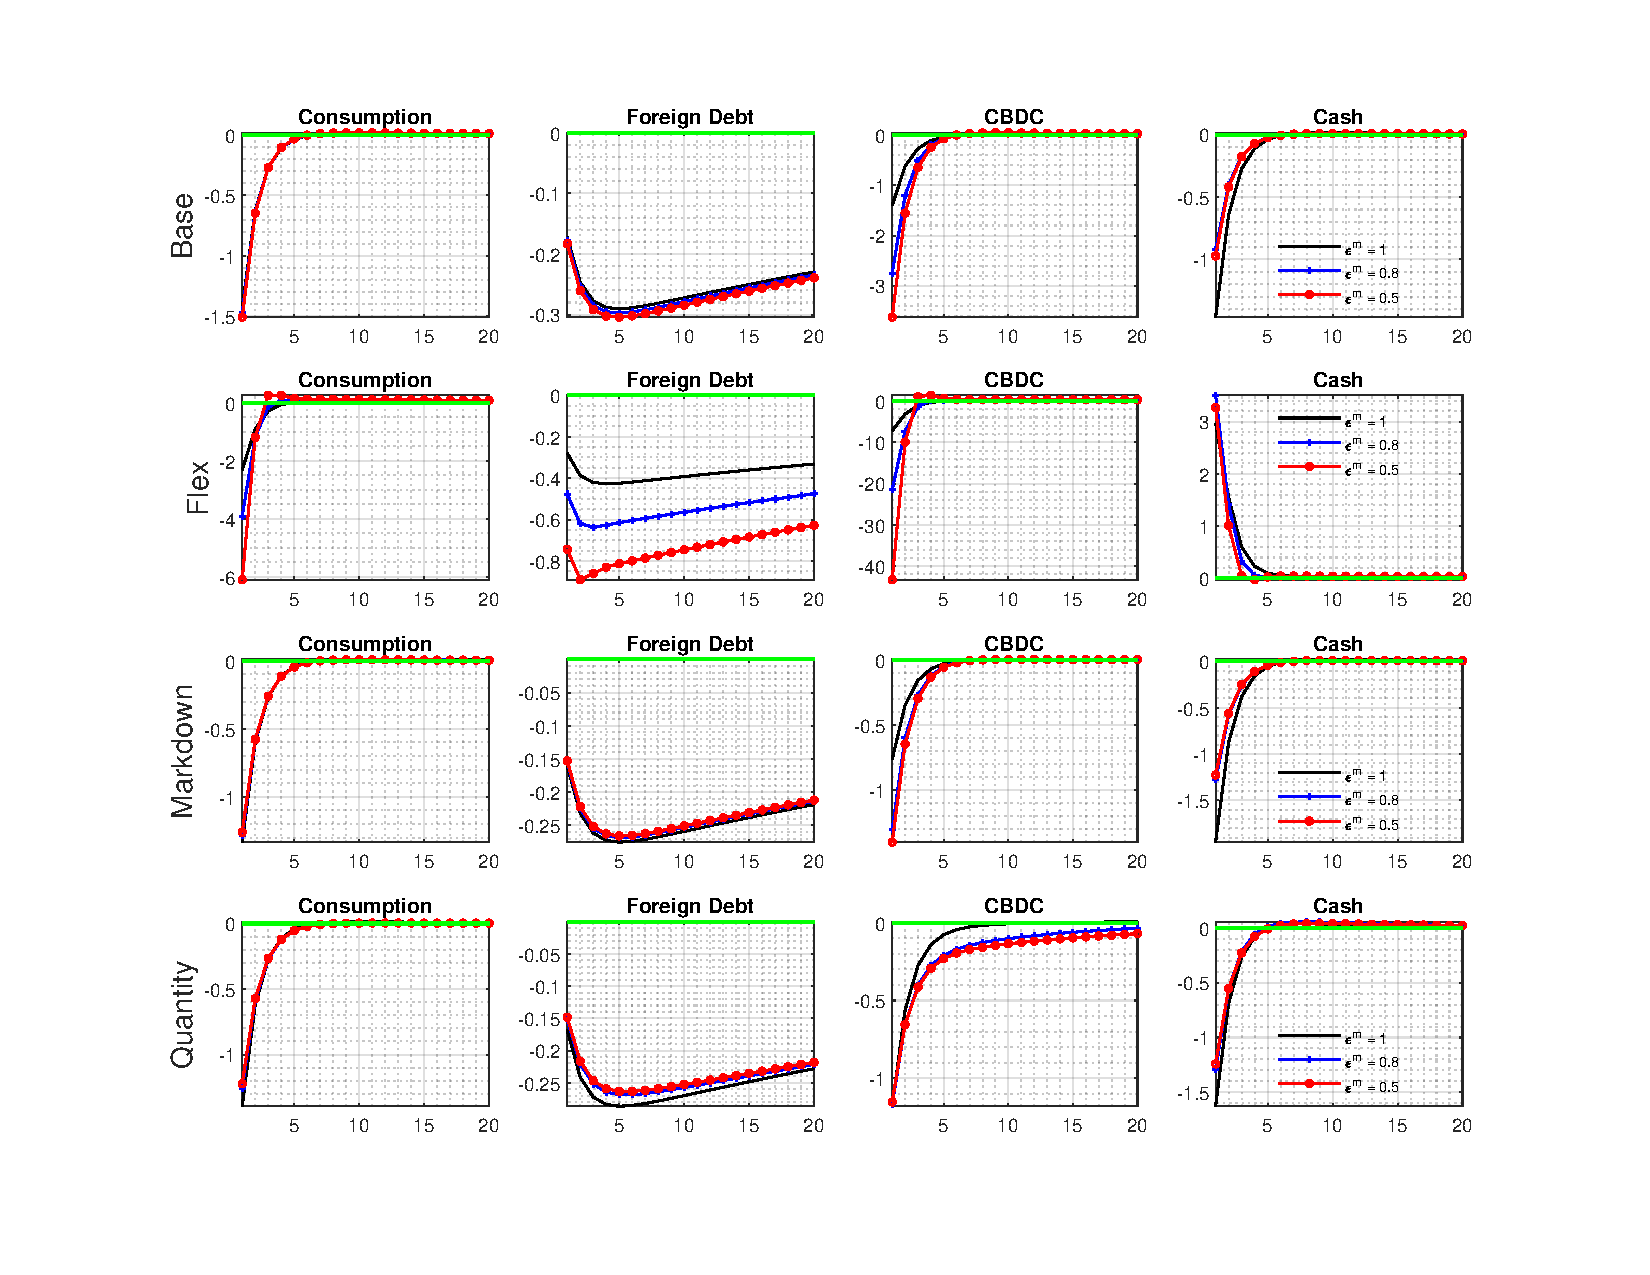
\includegraphics[trim = 0mm 23mm 0mm 18mm, clip, scale=0.93]{monetary_sto.pdf}}
	\caption{Response of selected variables to a 25 basic point tightening monetary policy shock in the domestic economy. All variables are expressed in percentage deviation from steady state.}
	\label{monalt_sto}
\end{figure}

\begin{figure}[H]
  \hspace{-0.1cm}
	\centering
	\centerline{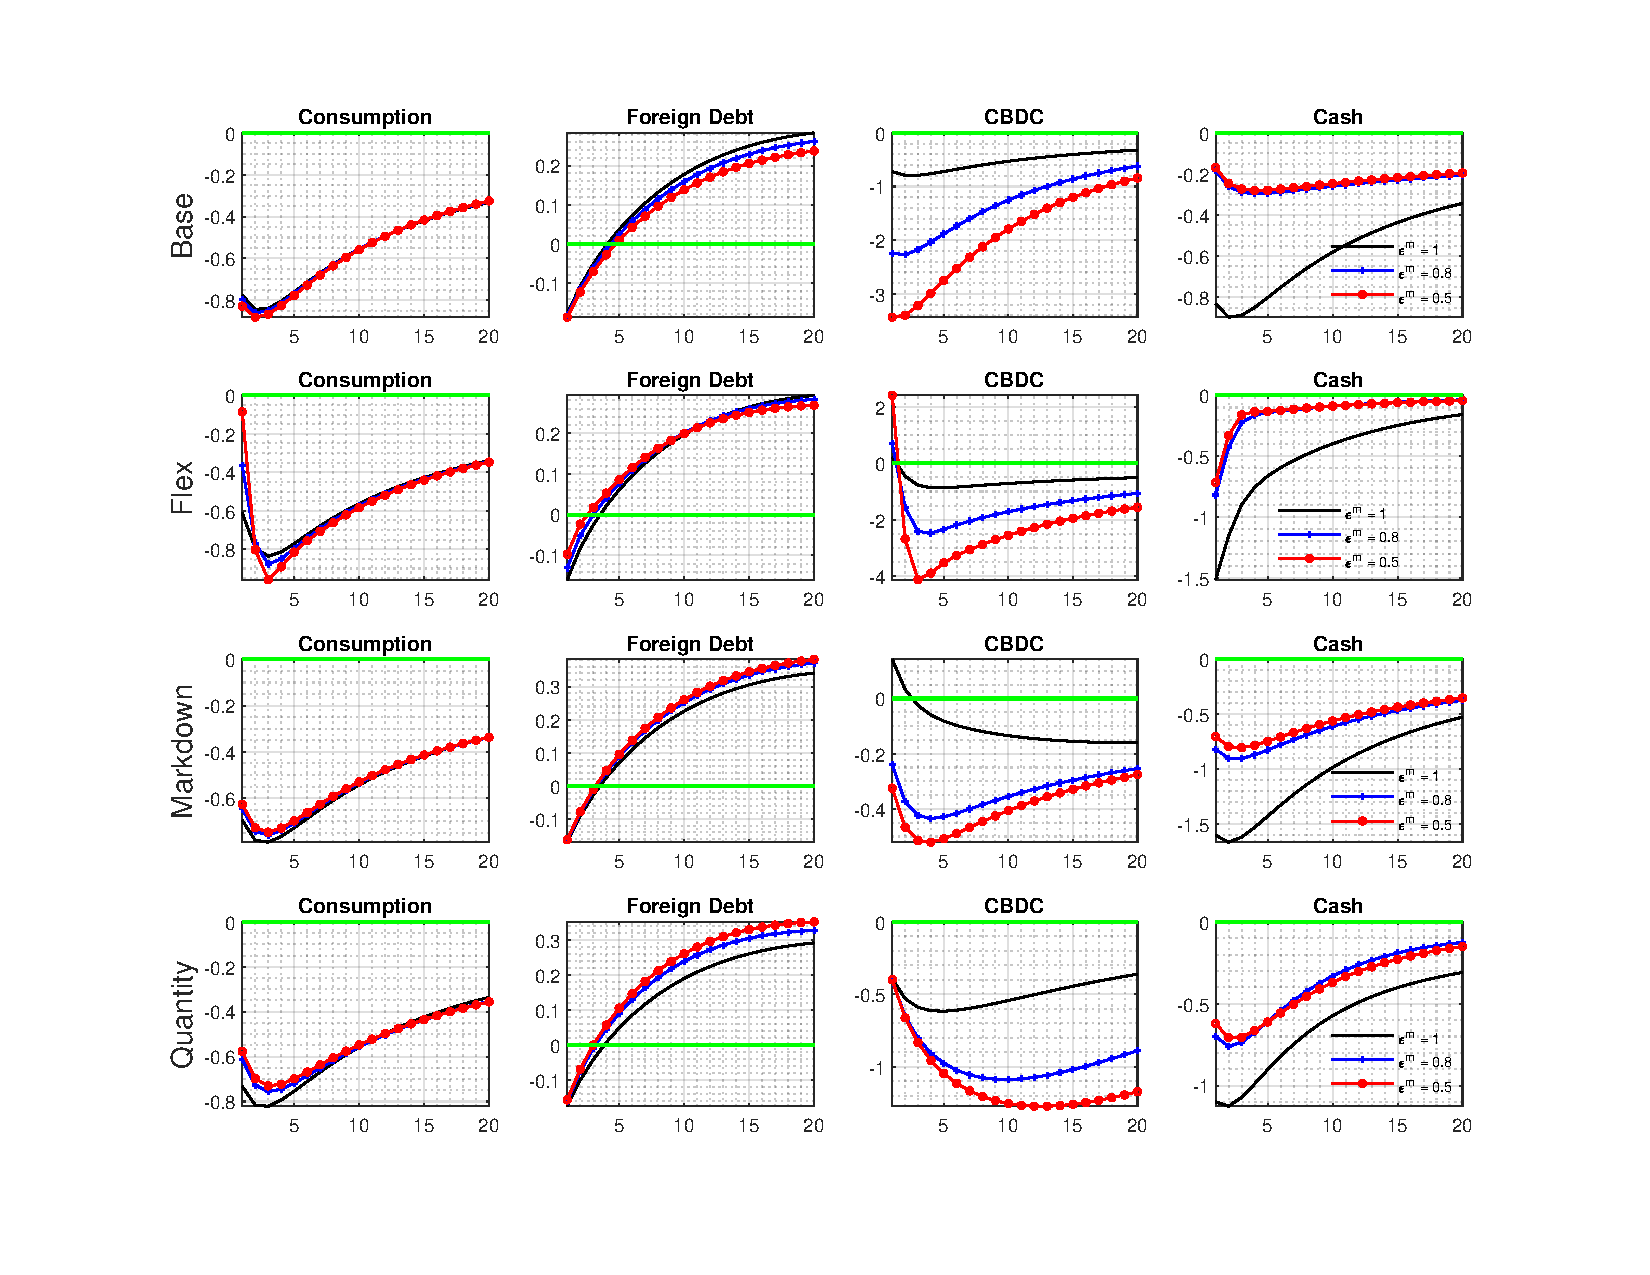
\includegraphics[trim = 0mm 23mm 0mm 18mm, clip, scale=0.93]{foreign_sto.pdf}}
	\caption{Response of selected variables to a one standard deviation expansionary foreign monetary policy shock in the domestic economy. All variables are expressed in percentage deviation from steady state.}
	\label{foralt_sto}
\end{figure}

\begin{figure}[H]
    \hspace{-0.1cm}
	\centering
	\centerline{\includegraphics[trim = 0mm 23mm 0mm 18mm, clip, scale=0.93]{TFP_liq.pdf}}
	\caption{Response of selected variables to a 1\% expansionary total factor productivity shock in the domestic economy. All variables are expressed in percentage deviation from steady state.}
	\label{TFP_liq}
\end{figure}
\begin{figure}[H]
  \hspace{-0.1cm}
	\centering
	\centerline{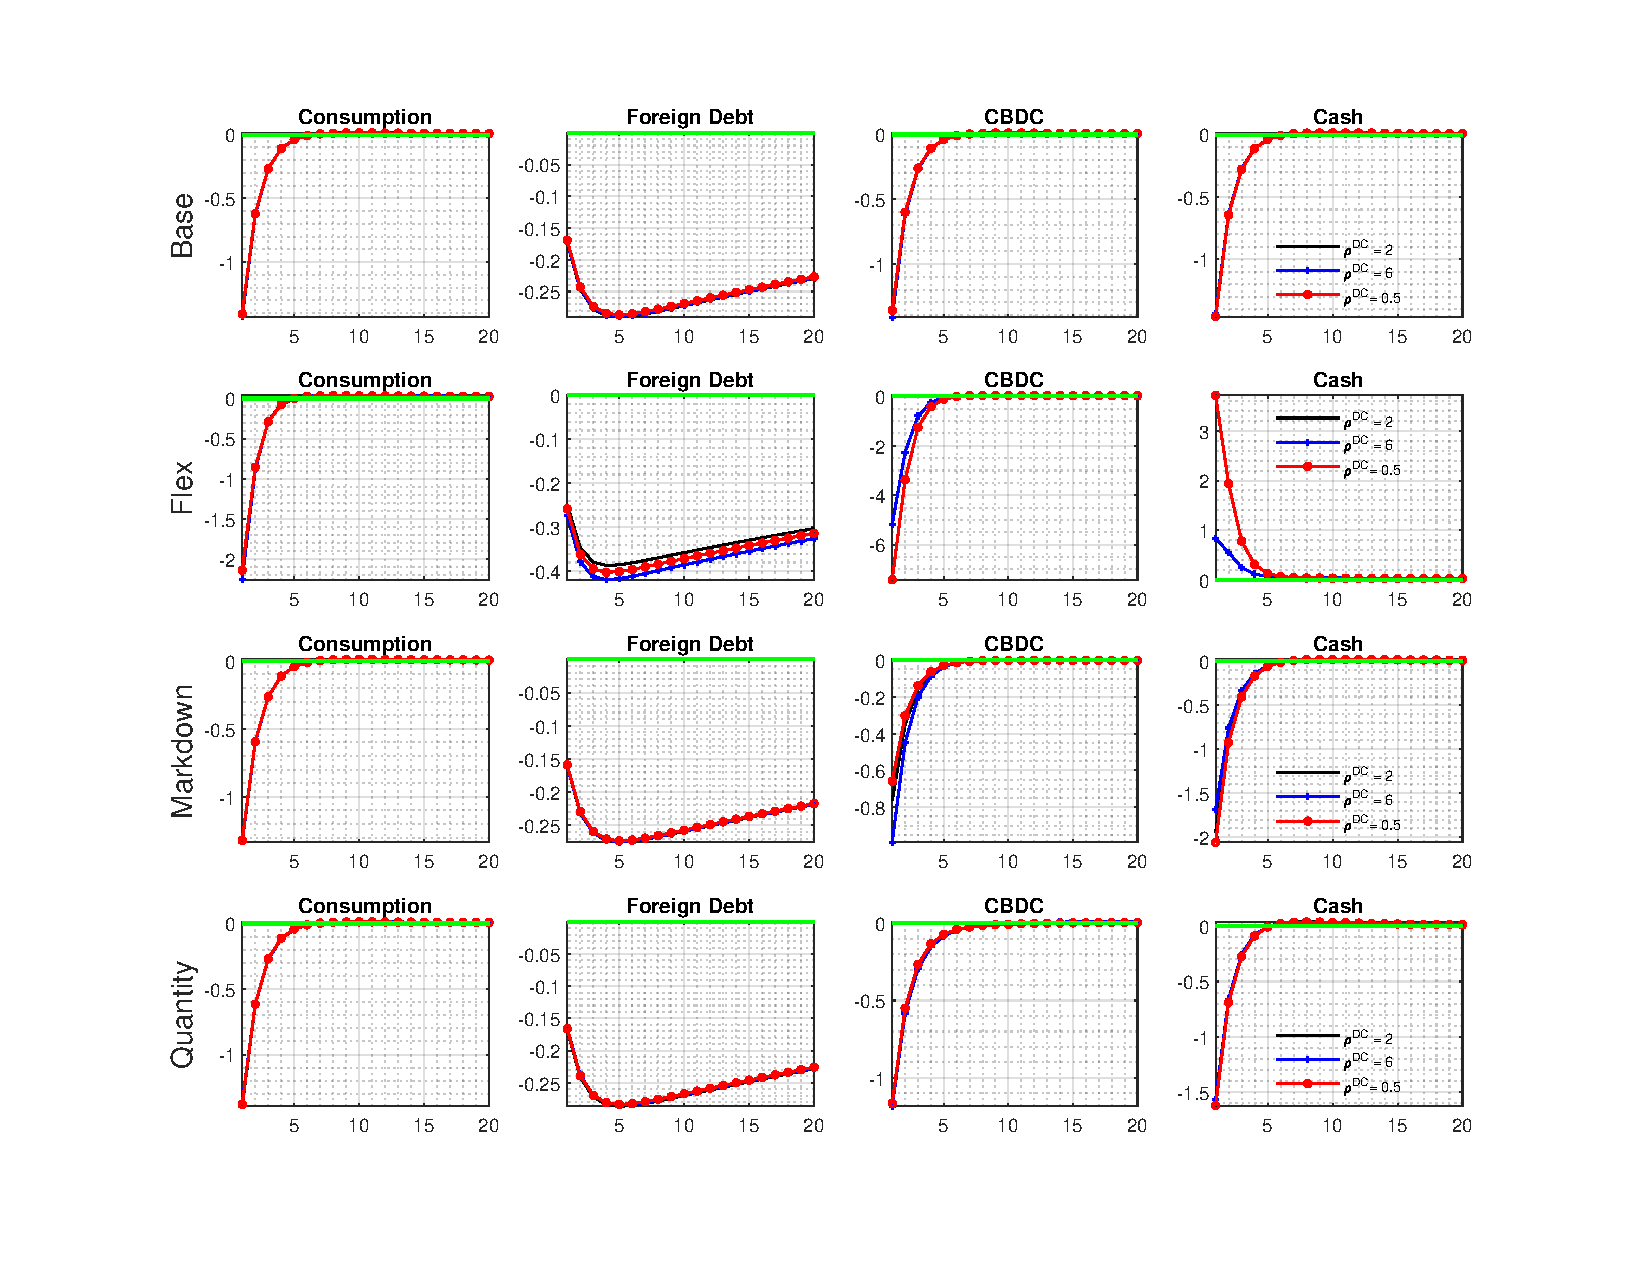
\includegraphics[trim = 0mm 23mm 0mm 18mm, clip, scale=0.93]{monetary_liq.pdf}}
	\caption{Response of selected variables to a 25 basic point tightening monetary policy shock in the domestic economy. All variables are expressed in percentage deviation from steady state.}
	\label{monalt_liq}
\end{figure}

\begin{figure}[H]
  \hspace{-0.1cm}
	\centering
	\centerline{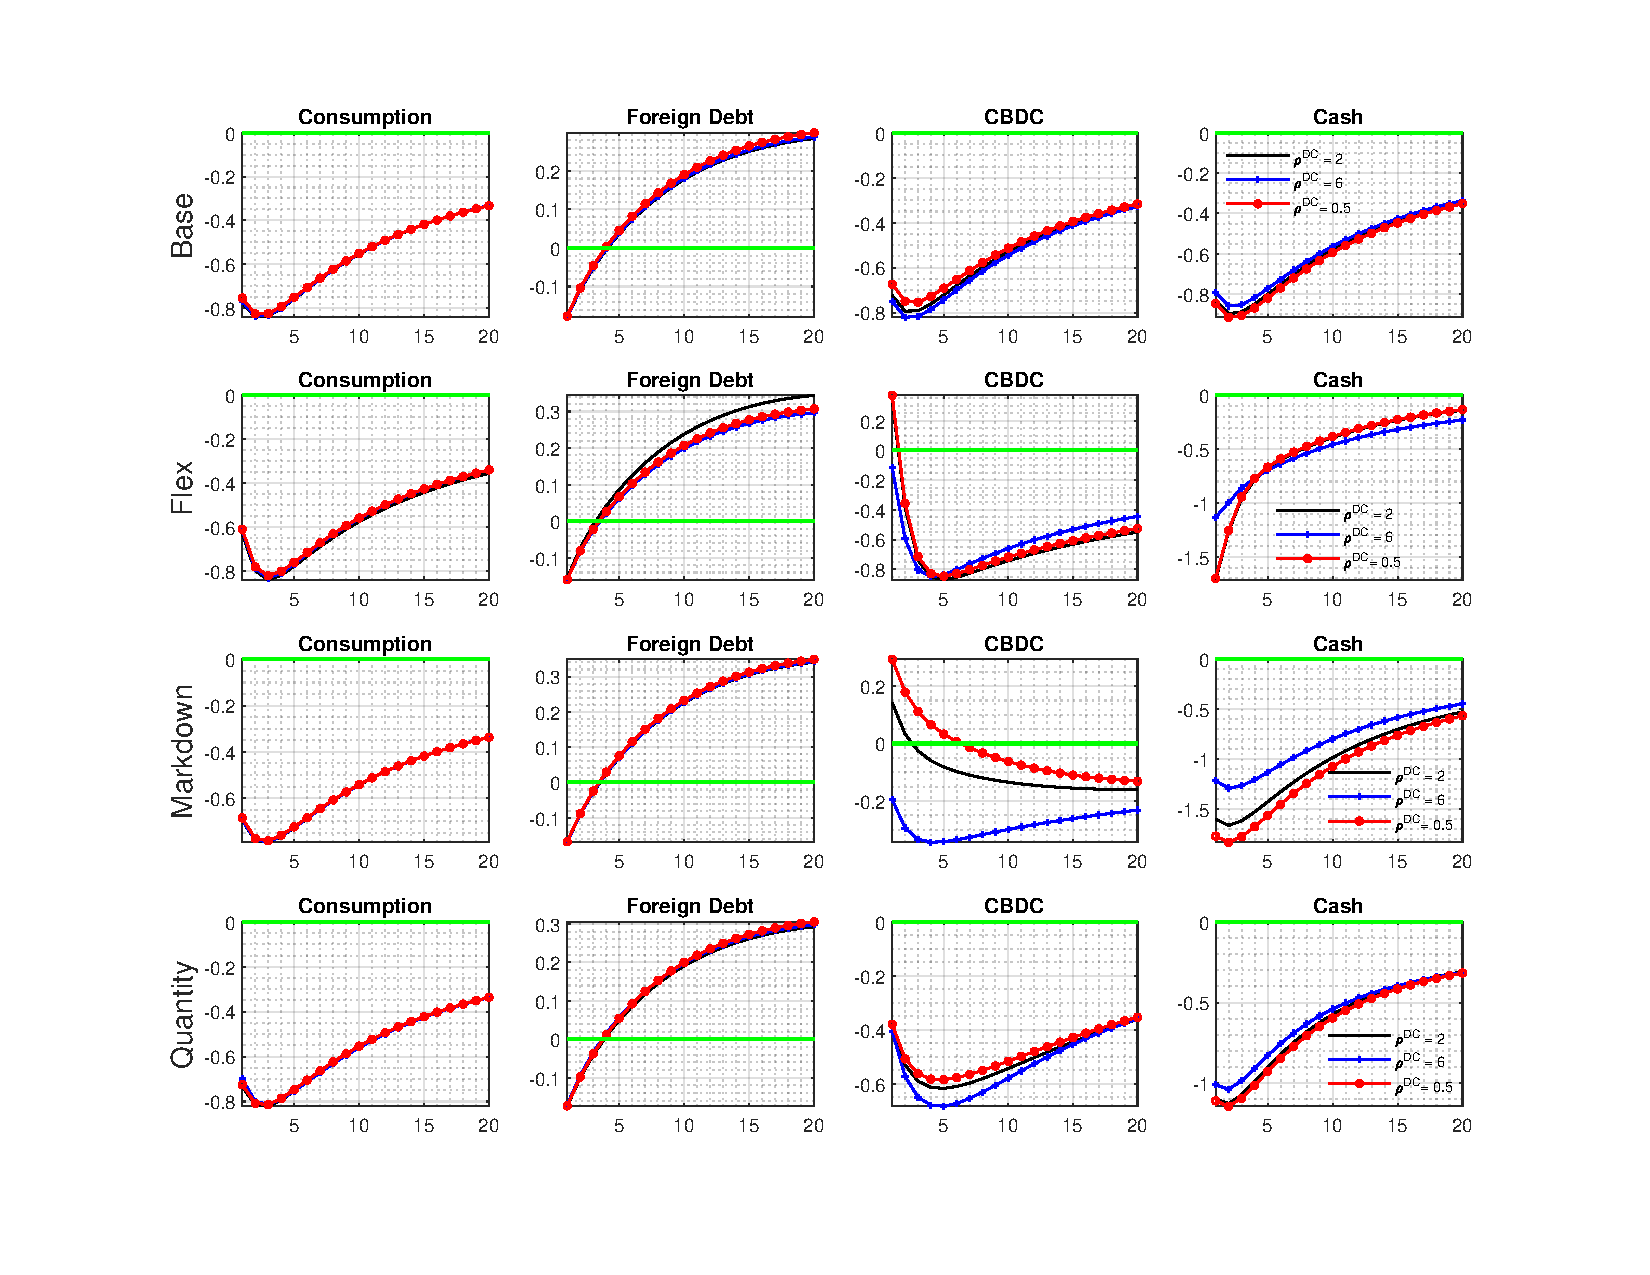
\includegraphics[trim = 0mm 23mm 0mm 18mm, clip, scale=0.93]{foreign_liq.pdf}}
	\caption{Response of selected variables to a one standard deviation expansionary foreign monetary policy shock in the domestic economy. All variables are expressed in percentage deviation from steady state.}
	\label{foralt_liq}
\end{figure}


\begin{table}[H]
\caption {\label{tab:table2} Variance Decomposition} 

\centering
\subcaption*{\bf{Cash}}
\begin{tabular}{llll}
 \hline
 &\textbf{R} & \textbf{A}  &  \textbf{$R^*$}  \\ 
 \hline
Consumption 	 & 	     3.86      &       55.36       &      40.77 \\
Inflation & 	  40.17      &       26.35       &      33.49  \\
Real FX & 	   0.92        &     59.60       &      39.48   \\
Foreign Debt	 & 	 3.88      &        0.23      &       95.89 \\
\hline
\end{tabular}
\centering
\subcaption*{\bf{Cash+CBDC}}
\begin{tabular}{llll}
 \hline
 &\textbf{R} & \textbf{A}  &  \textbf{$R^*$}  \\ 
 \hline
Consumption 	 & 	       3.90   &          55.32       &      40.78    \\
Inflation & 	  40.35    &         26.36      &       33.29      \\
Real FX & 	    0.92       &      59.49        &     39.59   \\
Foreign Debt	 & 	   3.95       &       0.22       &      95.82   \\
\hline
\end{tabular}
\centering
\subcaption*{\bf{Cash+Crypto}}
\begin{tabular}{llll}
 \hline
 &\textbf{R} & \textbf{A}  &  \textbf{$R^*$}  \\ 
 \hline
Consumption 	 & 	        4.66       &      77.28       &      18.06    \\
Inflation & 	    45.30      &       29.88       &      24.82     \\
Real FX & 	   1.39     &       72.91    &         25.69    \\
Foreign Debt	 & 	    23.21     &         9.77       &      67.02     \\
\hline
\end{tabular}

\centering
\subcaption*{\bf{Cash+Crypto+CBDC (Base)}}
\begin{tabular}{llll}
 \hline
 &\textbf{R} & \textbf{A}  &  \textbf{$R^*$}  \\ 
 \hline
Consumption 	 & 	          5.21     &        76.41      &       18.38     \\
Inflation  & 	   47.43      &       29.87        &     22.70      \\
Real FX  & 	      1.38        &     71.81        &     26.80     \\
Foreign Debt	 & 	   32.92    &          7.02        &     60.05   \\
\hline
\end{tabular}


\end{table}

\end{document}

